\documentclass[11pt]{gsasthesis} % 10,11 and 12pt fonts allowed

%%%%%%%%%%%%%%%% PACKAGES YOU PROBABLY WANT %%%%%%%%%%%%%%%%
% Include packages you want. The gsasthesis style file already includes
% packages "setspace" and "tocbibind".

% Included in original document
\usepackage{etex} % extend the number of registers

% GSAS: "all margins should be at least 1 inch."
\usepackage[margin={1.0in}]{geometry}
% If you want asymmetric margins for two-sided documents, use the "twoside" option, as in
% \usepackage[top=1in,bottom=1.5in,left=1in,right=1.5in,twoside]{geometry} 
% The left and right options become inner and outer margins 
% The default horizontal latex margin ratio is 2:3. The default vertical top:bottom margin ratio is 2:3 also. 
% You can also set it directly by passing the hmarginratio option to the geometry package, as in
% \usepackage[top=1in,left=1in,vmarginratio=2:3,hmarginratio=2:5,twoside]{geometry}

% Appendix package. Not necessary, but it does make managing appendices easier
\usepackage[titletoc]{appendix}

%%%%%%%%%%%%%%%% PACKAGES MAY WANT %%%%%%%%%%%%%%%%

% sideways tables and figures
\usepackage{rotating}

% tables that spill over multiple pages
\usepackage{longtable}

% references
% \usepackage{natbib}

% fonts that are nicer than defaults
\usepackage[sc]{mathpazo}
\usepackage{courier}

% Use 8-bit encoding that has 256 glyphs, pretty please
\usepackage[utf8]{inputenc}
\usepackage[T1]{fontenc}

% babel is required for blindtext, which generates random text
\usepackage[english]{babel}
\usepackage{blindtext}

% Slightly tweak font spacing for aesthetics
\usepackage{microtype}

% You need the footmisc package with the stable option if you want to have footnotes inside section titles, 
% for example to say that a particular chapter has been co-authored with someone. 
% The multiple option ensures that there is a comma between two consecutive footnotes
\usepackage[stable,multiple]{footmisc}

% Nicer captions
\RequirePackage[font=small,format=plain,labelfont=bf,textfont=it]{caption}
\addtolength{\abovecaptionskip}{1ex}
\addtolength{\belowcaptionskip}{1ex}

%%%%%%%%%%%%%%%% MSE Packages %%%%%%%%%%%%%%%%
% Base packages
\usepackage{fancyhdr}
\usepackage{amsmath}
\usepackage{amssymb}
\usepackage{geometry}
\usepackage{amsfonts}
\usepackage{mathtools}
\usepackage{setspace}
\usepackage{makecell}
\usepackage{amstext}
\usepackage{framed}
\usepackage{caption}
\usepackage{nicefrac}
\usepackage{xcolor}
\usepackage{listings}
\usepackage{verbatim}
\usepackage{soul}
\usepackage{gensymb}

% Inline Graphics
\usepackage{graphicx,float,subfig, grffile}
\graphicspath{
	{../figs/}
	{../figs/web/}
	{../figs/integration_test/planets/}
	{../figs/integration_test/asteroids/}
	{../figs/misc/}
}

% Captions
\captionsetup[figure]{font=small}

% MSE Terminal environment for screenshots
\lstdefinestyle{Terminal}
{
    basicstyle=\fontsize{8}{10}\color{black}\ttfamily
}

% MSE Code snippets
\lstdefinestyle{CodeSnippet}
{
    basicstyle=\linespread{1.0}\fontsize{10}{12}\color{black}\ttfamily
}
% MSE Macros
\newcommand{\tty}[1]{\texttt{#1}}

% Hypertext References
\usepackage{hyperref,color,textcomp}
\definecolor{webgreen}{rgb}{0,.35,0}
\definecolor{webbrown}{rgb}{.6,0,0}
\definecolor{RoyalBlue}{rgb}{0,0,0.9}
\definecolor{purp}{rgb}{0.6,0.3,0.9}
\hypersetup{
   colorlinks=true, linktocpage=true, pdfstartpage=3, pdfstartview=FitV,
   breaklinks=true, pdfpagemode=UseNone, pageanchor=true, pdfpagemode=UseOutlines,
   plainpages=false, bookmarksnumbered, bookmarksopen=true, bookmarksopenlevel=1,
   hypertexnames=true, pdfhighlight=/O,
   urlcolor=webbrown, linkcolor=RoyalBlue, citecolor=webgreen,
   pdfauthor={Michael S. Emanuel},
   pdfsubject={Harvard IACS Masters Thesis (May 2020)},
   pdfkeywords={},
   pdfcreator={pdfLaTeX},
   pdfproducer={LaTeX with hyperref}
}
\hypersetup{pdftitle={Kepler's Sieve}}


%%%%%%%%%%%%%%%% COMPULSORY FIELDS %%%%%%%%%%%%%%%%

\title{Kepler's Sieve: \\Learning Asteroid Orbits from Telescopic Observations} % needs to match title on DAC
\author{Michael S. Emanuel} % full name as it appears on your GSAS record, needs to match name on DAC
\degreename{Master of Science}
\degreefield{Data Science} % Official name of subject as listed in GSAS handbook
\department{Institute of Applied Computational Science} % official name of department
\degreemonth{May} % Month of Defense (i.e. month when DAC was signed)
\degreeyear{2020} % Year the DAC was signed
\principaladvisor{Professor Pavlos Protopapas}

% Optionally, you can add a second advisor, but you can't have three
\secondadvisor{Professor Christopher H. Rycroft}

% Macro definitions
\newcommand{\N}{\mathbb{N}}
\newcommand{\Z}{\mathbb{Z}}
\newcommand{\Q}{\mathbb{Q}}
\newcommand{\R}{\mathbb{R}}
\newcommand{\B}{\mathbb{B}}
\newcommand{\mcL}{\mathcal{L}}
\newcommand{\hamiltonian}{\mathcal{H}}
\newcommand{\p}{\partial}
\newcommand{\qvec}{\mathbf{q}}
\newcommand{\qearth}{\mathbf{q}_{\mathrm{Earth}}}
\newcommand{\qast}{\mathbf{q}_{\mathrm{Ast}}}
\newcommand{\vvec}{\mathbf{v}}
\newcommand{\uvec}{\mathbf{u}}
\newcommand{\xvec}{\mathbf{x}}
\newcommand{\Lvec}{\mathbf{L}}
\newcommand{\hvec}{\mathbf{h}}

\DeclarePairedDelimiter\norm{\lVert}{\rVert}

% MSE command to mark TODO items
\newcommand\todo[1]{\textbf{\textcolor{red}{#1}}}

\begin{document}

%%%%%%%%%%%%%%%% FRONTMATTER %%%%%%%%%%%%%%%%

\pagenumbering{roman} % GSAS wants roman page numbers for frontmatter

% the following four pages are required in that order. The first two pages are
% not allowed to have page numbers, this is taken care of in the class file.
\thesistitlepage
\copyrightpage
\begin{abstract}
% An abstract should be less than 350 words.
A novel method is presented to learn the orbits of asteroids from a large data set of telescopic observations.
The problem is formulated as a search over the six dimensional space of Keplerian orbital elements.
Candidate orbital elements are initialized randomly.
An objective function is formulated based on log likelihood that rewards candidate elements for getting 
very close to a fraction of the observed directions.
The candidate elements and the parameters describing the mixture distribution are jointly optimized using gradient descent.
Computations are performed quickly and efficiently on GPUs using the TensorFlow library.

The methodology of predicting the directions of telescopic detections is validated by demonstrating 
that out of approximately 5.69 million observations from the ZTF dataset,
3.75 million (65.71\%) fall within 2.0 arc seconds of the predicted directions of known asteroids.
The search process is validated on known asteroids by demonstrating the successful recovery 
of their orbital elements after initialization at perturbed values.
A search is run on observations that do not match any known asteroids.
I present orbital elements for [5] new, previously unknown asteroids.\\
\todo{Exact number of new asteroids presented}\\
All code for this project is publicly available on GitHub at \href{https://github.com/memanuel/kepler-sieve}{github.com/memanuel/kepler-sieve}.

\end{abstract}

% Center headings for table of contents, LOT, and LOF and make them smaller so that "Abstract", "Acknowledgments" and "Contents" all look alike. 
% Comment out if you want the default. If you want more control, use the "tocloft" package.
\renewcommand{\contentsname}{\protect\centering\protect\Large Contents}
\renewcommand{\listtablename}{\protect\centering\protect\Large List of Tables}
\renewcommand{\listfigurename}{\protect\centering\protect\Large List of Figures}

\tableofcontents % Table of contents

% The rest of the front matter: Lists of tables, figures, dedication and acknowledment is optional. 
% Comment out whatever you don't like
% \listoftables
% \listoffigures
\begin{acknowledgments}
I would like to thank my advisor, Pavlos Protopapas, for suggesting this topic and for his consistent support, advice and encouragement. \\
I would like to thank Chris Rycroft, my secondary advisor, for guiding me through a paper in Applied Math 225 in which I explored
numerical integrators for solving solar system orbits.\\
I would like to thank Matt Holman and Matt Payne from the Center for Astrophics (CFA) for their advice on state of the art solar system integrators.\\
Most importantly, I would like to thank my wife Christie and my children Victor and Ren\'ee for their love and support.
The Covid-19 crisis struck just as my work on this thesis kicked into high gear.
It would not have been possible to complete it without extraordinary understanding and support from them.
\end{acknowledgments}
% \begin{dedication}
%   To my parents
% \end{dedication}


%%%%%%%%%%%%%%%% MAIN BODY %%%%%%%%%%%%%%%%
\pagenumbering{arabic} % reset page numbering and switch to arabic

% Introductory chapter. Comment out if you don't have an intro chapter, but I think most committees expect you to have one.
% Don't number the intro chapter, but add to to the table of contents

% \addcontentsline{toc}{chapter}{Introduction}
% \chapter*{Introduction}\label{ch:intro}
% Determining the orbits of asteroids is one of the oldest problems in astronomy.
Classical methods are based on taking multiple observations of the same body through a telescope.
For an object that is large and bright enough, the human eye can ascertain the continuity of the motion,
i.e. that the data are multiple sightings of the same object.
Once enough sightings have been obtained, orbital elements can be solved using traditional
numerical methods, such as a least squares fitting procedure that seeks elements to minimize
the sum of squares error to all of the observations.

State of the art techniques for solving this problem are remarkably similar in spirit to the classical method.
Indeed, the first interstellar object, `Oumuamua, was discovered when astronomer Robert Weryk
saw it in images captured by the Pan-STARRS1 telescope on Maui.
\footnote{\href{https://en.wikipedia.org/wiki/\%CA\%BBOumuamua}{Wikipedia - Oumuamua}}
\footnote{\href{https://www.nytimes.com/2017/10/27/science/interstellar-object-solar-system.html}{NY Times - Astronomers Race to Study a Mystery Object from Outside the Solar System}}
More automated methods also exist.
Still, these methods are based on a search in the space of the observable data attributes: the time of observation (MJD), the right ascension (RA) and declination (DEC).
The apparent magnitude or brightness (MAG) is the third important observed quantity available for telescopic detections.
Two observations made close together in time at two points in the sky very near to each other have a relatively high probability of belonging to the same object.
Such a pair of observations is called a ``tracklet.''
Today's most automated approaches to identifying new asteroids from telescopic data are based on performing a greedy search of the observed data to extend tracklets.
Once a tracklet is identified, the algorithm attempts to extrapolate the path where future detections of this object might be.
After enough detections are strung together, a fitting procedure is tried to determine the orbital elements.

This is a solid technique and I do not mean to cast aspersion on it.
In this paper, however, I propose a new method which I believe has some significant advantages.
Rather than searching in the space of the data, i.e. (MJD, RA, REC, MAG), I propose to instead search over the six dimensional space of 
Keplerian orbital elements $(a, e, i, \Omega, \omega, f)$.
Why should we complicate things by searching implicitly, as it were, on the space of possible orbits,
rather than the simpler and more direct method currently used?
The main reason is to avoid a combinatorial explosion.

If you limit your search to candidate tracklets where you detect the same object multiple times in a short span of time,
you are going to miss any object that you detect only once or twice on a given night of observations.
But if this same object were seen on multiple nights, possibly separated over multiple days or longer, 
it becomes very costly to propose enough candidate tracklets to pick them up.
Indeed, you will soon face a combinatorial explosion in the number of possible tracklets.
A simplified model of the number of tracklets might be that we have a data set containing 
observations with a uniform density $\rho$ per day per degree squared of sky,
and we set a threshold $\tau$ in time and $\Delta$ in angular distance for how close a second observation must be to mark it as a candidate tracklet.

Here is a simple model showing the quadratic cost of enumerating candidate tracklets. \\
If you extend this further to tracks with 3 observations, the scaling gets even worse (cubic).\\
Let $\rho$ be the average density of detections per day per degree of sky.\\
Let $T$ be the number of days of observations in our data set.\\
Let $\tau$ be the threshold in days for 2 observations to be considered close enough in time to form a candidate tracklet.\\
Let $\Delta$ be the threshold angular distance in degrees for 2 observations to be considered close in the sky to form a candidate tracklet.\\
Let $A = 41,253$ be the number of square degrees in the sky.
\footnote{\href{https://en.wikipedia.org/wiki/Square_degree}{Wikipedia - Square Degrees in the Sky}}\\
Let $N = T \cdot A \cdot \rho $ be the total number of detections in the data set.\\
Let $\displaystyle{m = \tau \cdot \pi \Delta^2 \cdot \rho}$ be the average number of observations that will be close enough
to each candidate starting point of a tracklet.\\
Let $\displaystyle{NT_{2} = \frac{N \cdot m}{2!} = \frac{\tau}{T} \cdot \frac{\pi \Delta^2}{A} \cdot \frac{\rho^{2}}{2!} }$ 
be the total number of candidate trackets of size $2$. \\
Let $\displaystyle{NT_{k} = \frac{N \cdot m^{k-1}}{k!} = \left( \frac{\tau}{T} \cdot \frac{\pi \Delta^2}{A} \right)^{k-1} \cdot \frac{\rho^{k}}{k!} }$ 
be the total number of candidate trackets of size $k$. \\
We can see the bad news right away.
The number of tracklets of size $k$, $NT_{k}$, scales as $\rho^{k}$.
And the factors in the denominator don't bail us out.  
The number of possible ways $m$ to extend a tracklet is going to be a large number well in excess of 1.

This is the principal motivation for searching in the space of orbital elements.
While it's a large 6 dimensional space, its size is fixed in relation to the amount of data we have.
To be more precise, the number of candidate orbital elements will scale with the number of \textbf{asteroids} $K$ we are trying to detect
rather than the much larger number of \textbf{detections} $N$ in our data set.
The cost of the search algorithm presented below scales linearly in the observation density $\rho$ for each candidate element analyzed.
The cost of the entire algorithm is therefore on the order of $N \cdot K$, with no explosion as you consider tracklets larger than 2.
The second major reason for searching in the space of orbital elements is that it permits the search algorithm to string together observations made far apart in time.
This is a capability that eludes searches based on tracklets.

I summarize here the key steps in the search algorithm.
The first step is to generate a set of candidate orbital elements.
This is done with a very simple approach, one which can almost certainly be improved on later: random initialization.
For four of the orbital elements, $a$, $e$, $i$, and $\Omega$, one of the $733,489$ catalogued asteroids is selected at random.
Its orbital elements are used to populate these four.
It is worth emphasizing that each element is initialized with a \textit{independent} random asteroid;
the four elements in this part will almost never match one of the known asteroids across all four elements.
The remaining two orbital elements, $M$ (mean anomaly) and $\omega$ (argument of periapsis), 
are sampled uniformly at random on the circle $[0, 2 \pi)$.
These are then converted to the representation using $(a, e, i, \Omega, \omega, f)$.

Once the candidate elements have been initialized, they are integrated numerically using the \tty{REBOUND} library.
This is considered to be the gold standard of their true orbits.
This initial integration is then used to filter the data set of ZTF observations to a subset that are relevant for searching for orbits.
A routine computes the direction $\uvec_{\mathrm{pred}}$ in the barycentric mean ecliptic (BME) reference frame
that an observer at a given observatory site on earth would have seen light leaving an object with the candidate elements at a given observation time (MJD).
This quantity is computed at each unique observation time in the ZTF data set.
A separate computation is performed once on all of the ZTF observations converting the observed triplets $(MJD, RA, DEC)$
into vectors $\uvec_{\mathrm{obs}}$, the direction of the observation in the BME frame.
The angular distance between the predicted and observed direction is computed.
A threshold (2.0 degrees) is applied, and all ZTF observations falling within this threshold are cached in memory of the search class.

During the main body of the search process, the elements will be adjusted by a small amount in each training round.
These perturbed elements will have their orbits evaluated using the Kepler two body model.
An implementation is performed on the GPU using TensorFlow that is fast and differentiable.
The ``ground truth'' numerically integrated orbit is used to provide an adjustment term 
so that the predicted orbits will match the true orbits exactly when the perturbation is zero.
The predicted orbit can therefore be considered to be a linearization of the true orbits based on the Kepler model.

The objective of the optimization function is based on the log likelihood of a statistical model for the 
distribution of distances between predicted and observed directions.
A lemma will demonstrate that for directions uniformly distributed on the sphere, the squared distance over the 
threshold distance would be uniformly distributed on the interval $[0, 1]$.
A mixture model is formulated, where the distance between every predicted and observed direction is modeled as a mixture of hits and misses.
The misses are distributed uniformly on $[0, 1]$.
The hits are distributed as a truncated exponential distribution.
The decay parameter $\lambda$ of this exponential process is associated with a resolution parameter $R$.
This model is equivalent to assuming that some fraction $h$ (for hits) of the detections are due to 
a real body with the candidate elements, and that the results of the detection will be normally distributed 
with a precision parameter equal to the resolution.
During the search process, the threshold parameter is also updated.
This dynamic threshold should not be confused with the original threshold of 2.0 degrees used to build the filtered training data.

The optimization process jointly optimizes the candidate orbital elements and three parameters in the mixture model:
the assumed number of hits $N_{h}$, the resolution $R$, and the threshold $\tau$. 
Intuitively, we want the model to gradually tighten its focus, and adjust the orbital elements so they hit as many observations as closely as possible.
But we \textit{don't} want the model to get ``faked out'' by trying to get the elements closer to observations that belong to \textit{other} asteroids.
The model needs some way to update probabilities that each observation is a hit or a miss, which it does using the mixture model.
Early on, the optimization will try to get close to the central tendency of the data set.
If the initialization was good, it will gradually tighten in the resolution and threshold parameters.
The gradients will encourage the model to adjust the candidate orbital elements so that some of the observations,
the ones it sees as highly probable hits, will be very close to what is predicted by the candidate elements.
The observations modeled as highly probable misses will hardly contribute to the gradients of the candidate elements.

In practice, the optimization is carried out in alternating stages.
In odd numbered stages, only the resolution parameters are tuned at a higher learning rate;
in even numbered stages, both the resolution and orbital elements are adjusted together at a slower learning rate.
There are some additional subtleties where the actual optimization function during the training of the mixture
parameters has a term to encourage the model to shrink the resolution and threshold parameters.
These will be discussed at greater length below.

As much as possible, I have sought to validate individual components of these calculations in isolation.
My numerical integration of the planets is validated against results from NASA JPL (Jet Propulsion Library)
using the superb Horizons system.
\footnote{
\href{https://ssd.jpl.nasa.gov/horizons.cgi}{NASA Horizons} \\
I cannot say enough good things about Horizons.
If you want an external ``gold standard'' of where an object in the solar system was or will be 
and a friendly user interface, Horizons is an excelent resource.}
I separately validated the numerical integration of the first 16 asteroids against positions and velocities obtained from Horizons.

The notion of a direction in space from an observer on Earth is typically reported in telescopic data using a right ascension and declination.
While these are convenient and standard for reporting observed data, they are not well suited to the approach taken here.
All directions are represented internally in this project as a unit vector $\uvec = (u_x, u_y, u_z)$ in the Barycentric Mean Ecliptic (BME) frame.
These calculations were validated in isolation by querying the Horizons system for both the positions of and directions to known asteroids.
It is vital that this calculation takes into account the finite speed of light.
Treating light travel as instantaneous leads to errors that are catastrophically large in this context, on scales in the arc minutes rather than arc seconds.

The end to end calculation of a direction from orbital elements was verified indirectly as follows.
I integrated the trajectories of all the known asteroids using a collection of orbital elements downloaded from JPL.
I then computed the nearest asteroid number to each ZTF asteroid, and the distance between the predicted direction and observed direction.
I reviewed the statistical distribution of these distances.
I observed that out of approximately 5.69 million observations from the ZTF dataset,
3.75 million (65.71\%) fall within 2.0 arc seconds of the predicted directions of known asteroids.
I took this as overwhelming evidence that these calculations were accurate.

To put this degree of precision in context, 1.0 arc second is a back of the envelope estimate of the 
precision with which a modern telescope can determine direection of an observation under ideal observational conditions.
\footnote{Discussion with Pavlos Protopapas}
If you were to use an approximation that observations were made at Earth's geocenter 
(i.e. you did not account for location of the observatorory on Earth's surface) 
you would already be making errors on the order of 3 arc seconds.
If you were to perform your calculations using the Sun's location as your coordinate origin rather than the solar system barycenter,
you would make errors larger than 1.0 arc second.
I know because I made both of these errors in earlier iterations before squeezing them out!

I tested the capabilities of the search process with an increasingly demanding set of search tasks.
The first three search tasks involved recovering the elements of known asteroids.
I took a batch of 64 asteroids that appeared most frequently in the ZTF data set.
These asteroids were represented between 148 and 194 times in the data, 
where hits here are counted at a threshold of 2.0 arc seconds as before.
Here is a summary of the tests I ran:
\begin{itemize}
\item Initialize search with correct orbital elements, but resolution $R = 0.5 \degree$ and threshold $\tau = 2.0 \degree$.
All 64 elements were recovered to a resolution of 3.0 arc seconds and 4.6E-6 AU, matching on 162 hits.
\item Initialize search with small perturbation applied to orbital elements; $a$ by $1.0\%$, $e$ by $0.25\%$, $i$ by $0.05 \degree$,
remaining angles $f$, $\Omega$ and $\omega$ by $0.25 \degree$.
42 of 64 elements were recovered to 18 arc seconds and 2.6E-4 AU, matching on 118 hits
\item Initialize search with large perturbation applied to orbital elements; $a$ by $5.0\%$, $e$ by $1.0\%$, $i$ by $0.25 \degree$,
remaining angles $f$, $\Omega$ and $\omega$ by $1.0 \degree$.
12 of 64 elements were recoverd to 32 arc seconds and 4.5E-4 AU, matching on 98 hits.
In some cases, a different (but correct) set of orbital elements was obtained;
the perturbation was so large the search found a different asteroid.
\item Initialize a search with \textbf{randomly initialized} orbital elements.
Search against the subset of ZTF observations within $2.0$ arc seconds of a known asteroid.
This search converged on one set of orbital elements matching a real asteroid on the first batch of 64 random candidates.
\end{itemize}
The last last test was significantly more demanding in that it did not rely on known orbital elements.

The work encompassed in the first three tests above can be seen as a way to indpendently validate a subset of the known asteroid catalogue.
It can efficiently associate a large number of telescope observations with known asteroids,
which could in turn be used to further investigate those asteroids.
Analysis might include refining their estimated orbital elements, 
fitting the $H-G$ model of brightness (magnitude), or identifying some of them for further investigation if they meet criteria of interest,
e.g. orbits that will approach near to Earth in the future.

The main thrust of this work, however, is not on refining the existing asteroid catalogue, it is finding new asteroids.
The final search I ran was against the subset of ZTF observations that did not match any of the known asteroids.
Random initializations for orbital elements were tried.
Most of these initializations fail to converge on elements with enough hits to match real asteroids in the data,
but a small number do successfully converge.
I have identified 9 candidate elements for potentially new asteroids with 8 or more hits.
I have verified that none of the orbital elements modeled for these asteroids 
are obvious matches in the known asteroid catalogue, though some are arguably close.
I have also done an ad-hoc review of the ZTF records to ensure that they are plausibly belonging to the same object.
I believe that at least some of these candidate elements may represent new and unkown asteroids, and plan to submit them to the 
\href{https://www.minorplanetcenter.net/iau/mpc.html}{Minor Planet Center} for possible classification.

The ultimate goal of this project is not to simply perform a one time search of a dataset to identify some new asteroids.
The goal is rather to create a tool that will be of enduring use to astronomy community for solving the problem of 
searching for new asteroids given large volumes of telescopic data.
To that end, I plan to consult with Matt Holman and his colleagues at the Minor Planet Center to see what refinements and improvements
would be required to upgrade this from a tool I can use to one that is of wider use to the astronomy community.

%%% Local Variables:
%%% mode: latex
%%% TeX-master: t
%%% End:


% \chapter{Integrating the Solar System}\label{ch:1}
% \section{Introduction}
\label{section_intro}
The calculation of planetary orbits is arguably the canonical problem in mathematical physics.
Isaac Newton invented differential calculatus while working on this problem, and used his theory of gravitation to solve it.
In the important special case that one body in the system is a dominant central mass,
and all other bodies are viewed as massless ``test particles'', then a simple closed form solution is possible.
This formulation of the gravitational problem is often called the \href{https://en.wikipedia.org/wiki/Kepler_problem}{Kepler Problem},
named after \href{https://en.wikipedia.org/wiki/Johannes_Kepler}{Johannes Kepler}.
Kepler first studied this problem and published his famous \href{https://en.wikipedia.org/wiki/Kepler\%27s_laws_of_planetary_motion}{three laws of planetary motion},
the first of which states that the planets move in elliptical orbits with the sun at one focus.
This is a surprisingly good approximation for the evolution of the solar system, and the basis for the efficient linearized search over orbital elements developed in this thesis.

The two body approximation is not, however, sufficiently accurate for a high precision model of the past and future positions of the known bodies in the solar system.
While the mass of the sun is much larger than that of the heaviest planet, Jupiter, the planets are sufficiently massive
(and often closer to each other and other bodies of interest) that gravity due to their mass must also be accounted for.
The modern approach to determining orbits in the solar system is to use numerical integrators of the differential equations of motion.

\section{The \tty{REBOUND} Library for Gravitational Integration}
\label{section_rebound}
\tty{REBOUND} is an open source library for numerically integrating objects under the influence of gravity.
It is available on \href{https://github.com/hannorein/rebound}{GitHub}.
It is a first rate piece of software and I would like to thank Matt Holman and Matt Payne for recommending it to me last year.
At the end of Applied Math 225, I wrote a research paper in which I learned to use this library, 
extensively tested it on the solar system, and used it to simulate the near approach of the asteroid Apophis to Earth that will take place in 2029.
In this project, I use \tty{REBOUND} as the ``gold standard'' of numerical integration.
Because of its important role, I describe below how the \tty{IAS15} integrator I selected works.
\footnote{\tty{REBOUND} provides a front end to use multiple integrators. In this project, I make exclusive use of the default \tty{IAS15} integrator.}

The \tty{IAS15} integrator, presented in a 2014 paper by Rein and Spiegel, is a an impressive achievement.
It a fast, adaptive, 15th order integrator for the N-body problem that is (amazingly!) 
accurate to machine precision over a billion orbits.  
The explanation is remarkably simple in comparison to what this algorithm can do.  
Rein and Spiegel start by writing the equation of motion in the form 
$$y'' = F[y', y, t]$$
Here $y$ is the position of a particle; $y'$ and $y''$ are its velocity and acceleration;
and $F$ is a function with the force acting on it over its mass.
In the case of gravitational forces, the only dependence of $F$ is on $y$; 
but one of the major advantages of this framework is its flexibility to support other forces,
including non-conservative forces that may depend on velocity.
Two practical examples are drag forces and radiation pressure.

This expression for $y''$ is expanded to 7th order in $t$, 
$$y''[t] \approx y_0'' + a_0t + a_1t^2 + \cdots +a_6 t^7$$
They next change variables to dimensionless units $h = t / dt$ and coefficients $b_k = a_k dt^{k+1}$:
$$y''[t] \approx y_0'' + b_0h + b_1h^2 + \cdots + b_6 h^7$$
The coefficients $h_i$ represent relative sample points in the interval $[0, 1]$ that subdivide a time step.
Rein and Spiegel call them substeps.  
The formula is rearranged in terms of new coefficients $g_k$ with the property that $g_k$ depends
only on force evaluations at substeps $h_i$ for $i \le k$.
$$y''[t] \approx y_0'' + g_1h + g_2h(h-h_1) + g_3h(h-h_1)(h-h_2) + \cdots + g_8 h (h-h_1) \cdots (h-h_7)$$
Taking the first two $g_i$ as examples and using the notation $y_n'' = y''[h_n]$,
$$g_1 = \frac{y_1'' - y_0''}{h_1} \quad\quad  g_2 = \frac{y_2'' - y_0'' -g_1h_2}{h_2(h_2-h_1)}$$
This idea has a similar feeling to the Jacobi coordinates: a change of coordinates
with a dependency structure to allow sequential computations.

Using the $b_k$ coefficients, it is possible to write polynomial expressions for $y'[h]$ and $y''[h]$:
\begin{align*}
y'[h] &\approx y_0' + h dt \left(y_0'' + \frac{h}{2}\left(b_0 + \frac{2h}{3}\left(b_1 + \frac{}{} \cdots \right)\right) \right) \\
y[h] &\approx y_0 + y_0' h dt + \frac{h^2dt^2}{2}\left(y_0'' + \frac{h}{3}\left(b_0 + \frac{h}{2}\left(b_1 + \frac{}{} \cdots \right)\right) \right)
\end{align*}

The next idea is to use \href{http://mathworld.wolfram.com/RadauQuadrature.html}{Gauss-Radau quadrature}
to approximate this integral with extremely high precision.  
Gauss-Radau quadrature is similar to standard Gauss quadrature for evaluating numerical integrals, 
but the first sample point is at the start of the integration window at $h=0$.
This is a strategic choice here because we already know $y'$ and $y''$ at $h=0$ from the previous time step.
This setup now reduces calculation of a time step to finding good estimate of the coefficients $b_k$.
Computing the $b_k$ requires the forces during the time step at the sample points $h_n$,
which in turn provide estimates for the $g_k$, and then feed back to a new estimate of $b_k$.

This is an implicit system that Rein and Spiegel solve efficiently using what they call a predictor-corrector scheme.
At the cold start, they set all the $b_k=0$, corresponding to constant acceleration over the time step.
This leads to improved estimates of the forces at the substeps, and an improved estimates for the path on the step.
This process is iterated until the positions and velocities have converged to machine precision.
The first two time steps are solved from the cold start this way.  

Afterwards, a much more efficient initial guess is made.  
They keep track of the change between the initial prediction of $b_k$ and its value after convergence,
calling this correction $e_k$.  At each step, the initial guess is $b_k$ at the last step plus $e_k$.
An adaptive criterion is used to test whether the predictor-corrector loop has converged.
The error is estimated as 
$$\widetilde{\delta b_6} = \frac{\max_i |\delta b_{6,i}|}{\max_i |y_i''|}$$
The index $i$ runs over all 3 components of each particle.
The loop terminates when $ \widetilde{\delta b_6} < \epsilon_{\delta b}$; they choose $\epsilon_{\delta b} = 10^{-16}$.
It turns out that the $b_k$ behave well enough for practical problems that this procedure will
typically converge in just 2 iterations!

The stepsize is controlled adaptively with an analogous procedure.
The tolerance is set with a dimensionless parameter $\epsilon_b$,
which they set to $10^{-9}$.
As long as the step size $dt$ is ``reasonable'' in the sense that it can capture
the physical phenomena in question, the error in $y''$ will be bounded by the last term
evaluated at $h=1$, i.e. the error will be bounded by $b_6$.
The relative error in acceleration $\widetilde{b_6} = b_6 / y''$ is estimated as
$$ \widetilde{b_6} = \frac{\max_i |b_{6,i}|}{\max_i |y_i''|}$$
These are similar to the error bounds for convergence of the predictor-corrector loop,
but involve the magnitude of $b_6$ rather than its change $\delta b_6$.
An immediate corollary is that changing the time step by a factor $f$ will change $b_6$
by a factor of $f^7$.

An integration step is computed with a trial step size $dt_{\text{trial}}$.
At the end of the calculation, we compute the error estimate $\widetilde{b_6}$.
If it is below the error tolerance $\epsilon_b$, the time step is accepted.
Otherwise, it is rejected and a new attempt is made with a smaller time step.
Once a time step is accepted, the next  time step is tuned adaptively according to
$dt_{\text{required}} = dt_{\text{trial}} \cdot \left( \epsilon_b / \widetilde{b_6}\right)^{1/7}$
Please note that while the relative error in $y''$ may be of order 7, 
the use of a 15th order integrator implies that 
shrinking the time steps by a factor $\alpha$ will improve the error by a factor of $\alpha^{16}$.

% Hein and Spiegel include an interesting discussion of the different sources of error in N-body integrators.
% They explore the familiar errors arising from the numerical scheme, 
% but also explore both random and biased numerical errors.
% They give a complete error decomposition
% $$E_{\text{tot}} = E_{\text{floor}} + E_{\text{rand}} + E_{\text{bias}} + E_{\text{scheme}}$$
% $E_{\text{floor}}$ is the baseline numerical error that is unavoidable when we try to represent
% real numbers to limited machine precision.
% $E_{\text{rand}}$ is the familiar errors due to accumulated numerical round-off, 
% provided they are distributed randomly (i.e. unbiased).  
% $E_{\text{bias}}$ is an accumulated effect of numerical round-off that has a bias.

% This is a subtle point best illustrated by an example.
% Suppose you have a floating point representation of a 2x2 rotation matrix.
% For a given angle $\phi$, the floating point sum of $\cos^2\phi + \sin^2\phi$
% is likely not to be 1.0 to full machine precision.  
% If it is even a tiny bit less than 1, then repeated application of this rotation matrix
% over many time steps will gradually lead to a contraction.
% Rein and Spiegel devote substantial effort to minimizing rounding errors, 
% particularly by using \href{https://en.wikipedia.org/wiki/Kahan_summation_algorithm}{compensated sums}.
% This simple idea adds only slightly to the run time but can lead to significant accuracy improvements,
% especially over long term simulation, e.g. on the order of one billion orbital periods.

% Rein and Spiegel test the phase accuracy of \tty{IAS15} by running integrating the 
% outer solar system forward in time for 50 orbits with a fixed time step,
% then backwards for 50 orbits with the same time step.
% The known answer is that the phases should be the same, allowing for sharp accuracy measurements.
% This test shows that \tty{IAS15} is more accurate than the comparisons including WH at preserving phases.

% They also introduce a criterion of optimality and demonstrate that \tty{IAS15} integrator satisfies it.
% A result called Brouwer's Law status that in the presence of round-off, 
% a cumulative sum will have have an error that scales as $n^{1/2}$, i.e. it is a random walk of $n$ steps.
% Angular type variables including the orbital phase grow as $n^{3/2}$.
% The authors tested \tty{IAS15} and other integrators on a long term integration of the outer solar system
% (Jupiter, Saturn, Uranus, Neptune) for one billion Jupiter orbits, approximately 12 billion years.
% The energy errors satisfied Brouwer's law, and grew more slowly than those made by the other schemes.
% One surprising conclusions is that the non-symplectic \tty{IAS15} integrator is ``more symplectic''
% (in the sense of having smaller energy errors) than the symplectic integrators!
% This is a completely non-obvious results, and shows the importance of analyzing and understanding
% all the sources of error in a calculation.

\section{A Brief Review of the Keplerian Orbital Elements}
\label{section_orbital_elements}
In his work on the two body problem and the orbits of the planets, Kepler defined six 
\href{https://en.wikipedia.org/wiki/Orbital_elements}{orbital elements}
that are still in use today.
A set of orbital elements pertains to a body as of a particular instant in time, which is typically referred to as the ``epoch'' in this context.
The data sources I've seen all describe the time as a floating point number in the \href{https://en.wikipedia.org/wiki/Julian_day}{Modified Julian Day} (mjd) format.
In particular, I obtained orbital elements for all the known asteroids from \href{https://ssd.jpl.nasa.gov/?sb_elem}{JPL small body orbital elements}
as of MJD 58600, corresponding to 27-Apr-2019 on the Gregorian calendar.\\
Here is a brief review of the definitions of these orbital elements

\begin{figure}
\begin{center}
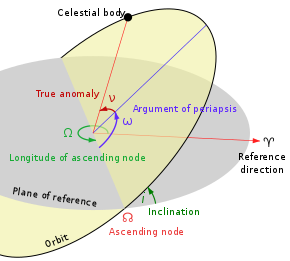
\includegraphics[width=0.40\textwidth]{orbital-elements-wikipedia.png}
\caption{Definition of the traditional Keplerian
\href{https://en.wikipedia.org/wiki/Orbital_elements}{orbital elements}
orbital elements, courtesy of Wikipedia.\\
Two parameters define the shape and size of the ellipse;
two define the orientation of the orbital plane; 
and the last two orient the ellipse in its plane and the phase of the body on its ellipse.}
\end{center}
\end{figure}

\begin{samepage}
\begin{itemize}
\item $a$, the semi-major axis; named \tty{a} in JPL and REBOUND
\item $e$, the eccentricity; named \tty{e} in both systems
\item $i$, the inclination; named \tty{i} in JPL and \tty{inc} in REBOUND
\item $\Omega$, the longitude of the ascending node; named \tty{node} in JPL and \tty{Omega} in REBOUND
\item $\omega$, the argument of perihelion; named \tty{peri} in JPL and \tty{omega} in REBOUND
\item $f$, the true anomaly; named \tty{f} in REBOUND; not quoted directly by JPL
\item $M$, the mean anomaly; named \tty{M} in both systems
\item mjd, the epoch as a Modified Julian Date
\end{itemize}
\end{samepage}
Distances are in A.U. in both JPL and REBOUND.  \\
Angles are quoted in degrees in JPL and in radians in REBOUND.

These orbital elements have stood the test of time because they are useful and intuitive.
They are ideal for computations, both theoretical and numerical, because in the case of the two body problem five of the six orbital elements remain constant.
The careful reader will note that there are 8 entries in the table above, but I've described elements as coming six at a time.
The epoch is considered to be the ``seventh element'' because in the Kepler two body problem, we can describe one body at different times, but it will have the same orbit.
This point of view extends to the N-body problem, which is fully reversible; the same system can be described at at different moments in time.
In practice, the orbital elements are often used to describe the initial conditions of all the bodies for an integration.
The problem is then integrated numerically, possibly both forwards and backwards.
Orbital elements can be reported for any body of interest.

A body orbiting the sun has six degrees of freedom.  
In Cartesian coordinates, there are three for the position and three for the velocity.
In orbital elements, the first five are almost always $(a, e, i, \Omega, \omega)$.
These five will remain constant for a body moving in the Kepler two body problem.

There is some variation in the choice of the sixth element, because different representations have different pros and cons.
The true anomaly $f$ is most convenient for transforming back and forth between orbital elements and Cartesian space.
The mean anomaly $M$ is most convenient for studying the time evolution of the system, because it changes linearly with time in the Kepler two body problem.
The mean anomaly and true anomaly are related by the famous 
\href{https://en.wikipedia.org/wiki/Kepler\%27s_equation}{Kepler's Equation}
This relates the mean anomaly $M$ to the eccentric anomaly $E$.
The \href{https://en.wikipedia.org/wiki/Eccentric_anomaly}{eccentric anomaly} is yet another angle describing a body in orbit.
\begin{figure}
\begin{center}
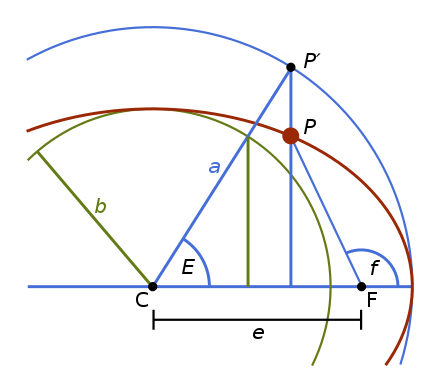
\includegraphics[width=0.40\textwidth]{orbital-anomalies.png}
\caption{Three Orbital Anomalies: Eccentric, Mean and True}
\end{center}
\end{figure}

\begin{align*}
\tan \left(\frac{f}{2} \right) &= \sqrt{\frac{1+e}{1-e}} \tan \left( \frac{E}{2} \right) \\
M &= E - e \sin(E)
\end{align*}
 
The linear evoluation of the mean anomaly, along with Kepler's equation, allows us to efficiently compute orbits for the Kepler two body problem.
The relationship between the eccentric anomaly $E$ and true anomaly $f$ is a one to one function that can be evaluated fast on a computer.
The mapping from eccentric anomaly $E$ to mean anomaly $M$ is also fast.
The inverse mapping from $M$ to $E$ does not have a known analytical form.
But it can be evaluated raplidly using Newton's Method with a reasonable initial guess.
This is the method that I use to compute the orbits under the Kepler approximation. 

\section{Numerical Integration of the Planets and Asteroids}
\label{section_numerical_integration}

I have described above a library \tty{REBOUND} that can efficiently integrate the solar system,
and a data source Horizons that can be used to obtain accurate initial conditions for solar bodies.
In principle integrating the solar system is a straightfoward exercise.
In practice, there are quite a few details that need to be worked out before you can obtain reliably correct answers.
You need to carefully specify the bodies you submit to Horizons.
Horizons has separate identifiers for e.g. the barycenter of the Earth-Moon system, the Earth, and the Moon.

The module \tty{horizons.py} contains functions used to query the Horizons AP.
It also maintains a local cache with the results of prior queries; 
this yields significant savings in time because a typical horizons query using the Horizons API in \tty{REBOUND} takes about one second.
The main function in this module is \tty{make\_sim\_horizons}.
Given a list of object names and an epoch, it queries Horizons for their positions and velocities as of that date.
It uses this data to instantiate a \tty{REBOUND Simulation} object. \\
The module \tty{rebound\_utils.py} contains functions used to work with \tty{REBOUND} simulations.
It includes functions to build a simulation (\tty{make\_sim}).
This will seek to load a saved simulation on disk if it is available, otherwise it will query Horizons for the required initial conditions.
The function \tty{make\_archive} builds a \tty{REBOUND SimulationArchive}.
As the name suggets, a \tty{SimulationArchive} is a collection of simulation snapshots that  have been integrated.
This function also saves the integrated positions of the planets and test bodies as plain old \tty{Numpy} arrays for use in downstream computations.

The module \tty{planets.py} performs the numerical integration of the planets.
To be more precise, it will integrate different collections of massive bodies in the solar system
\begin{itemize}
\item \textbf{Planets}: The Sun; The Earth and Moon as separate bodies; and the barycenters of the other seven IAU planets 
Mercury, Venus, Mars, Jupiter, Saturn, Uranus, and Neptune (10 objects)
\item \textbf{Moons}: The 8 IAU planets, plus the following significant moons and Pluto (31 objects): \\
Jupiter: Io, Europa, Ganymede, Callisto \\
Saturn: Mimas, Enceladus, Tethus, Dione, Rhea, Titan, Iapetus, Phoebe \\
Uranus: Ariel, Umbriel, Titania, Oberon, Miranda \\
Neptune: Triton, Proteus \\
Pluto: Charon 
\item \textbf{Dwarfs}: All objects in the solar system with a mass at least $1E-10$ Solar masses (31 objects): \\
Planets: Earth, Moon, and barycenters of other seven planets \\
Above 1E-9: Pluto Barycenter, Eris, Makemake, Haumea \\
Above 1E-10: 2007 OR10, Quaoar, Hygiea, Ceres, Orcus, Salacia, Varuna, Varda, Vesta, Pallas
\item \textbf{All}: All objects in the solar system with a mass at least $1E-10$ Solar masses (45 objects): \\
All 8 planets (not barycenters) \\
All the heavy moons above \\
All the dwarf planets above
\end{itemize}

Each configuration above was integrated for a 40 year period spanning 2000-01-01 to 2030-12-31 and a time step of 16 days.
I tested the integration by comparing the predicted positions of the 8 planets to the position quoted by Horizons at a series of test dates .
The test dates are at 1 year intervals over the full 40 year span that is simulated.
The best results were obtained by integrating smallest collection: Earth, Moon, and the barycenters of the other 7 planets.
I was a bit surprised at this result and expected to do slightly better as the collection of objects became larger.
Position errors are reported in AUs, with the root mean square (RMS) error over the 40 annual dates.
I also compute an angle error by comparing the instantaneous direction from each planet to Earth geocenter in the BME frame.
I reported errors on this basis because on this problem, everything is done in terms of directions so precision eventually
comes down to a tolerance in arc seconds.

\begin{table}
\begin{centering}
\begin{tabular}{ | c | c | c |}
\hline
\multicolumn{1}{|p{2cm}|}{\centering Object \\ Collection } & 
\multicolumn{1}{|p{2cm}|}{\centering Position \\ Error} & 
\multicolumn{1}{|p{2cm}|}{\centering Angle \\ Error} \\
\hline
Planets & 5.38E-6 & 0.79 \\
Moons & 1.35E-5 & 0.81 \\
Dwarfs & 5.38E-6 & 0.79\\
All & 1.35E-5 & 0.81 \\
\hline
\end{tabular}
\caption{Root Mean Square Error in Integration of Planets vs. Horizons\\
Position Error: RMS error of 8 planets in AU.\\
Angle Error: RMS error in direction from planet to Earth geocenter, in Arc Seconds}
\end{centering}
\end{table}

While it might at first seem surprising that the results are worse for the more complex integrations including the moons,
it's important to realize that this problem is intrinsically more difficult.
Simulating the evolution of the barycenter of e.g. the Jupiter system is significantly easier than keeping track of the heavy moons and integrating them separately.
Overall these results are excellent; over a span of 20 years in either direction, integrations are accurate on the order of $10^{-6}$ AU.
The angular precision on the order of $\sim 0.8$ arc seconds is also excellent for such a long time span and well within the tolerance of this application.

After reviewing these results, I decided that the optimal strategy for the asteroid search problem was to treat the heavy bodies 
in the solar system as the smallest collection, shown on row 1.
It is necessary to model the position of the Earth and Moon separately rather than the Earth-Moon barycenter, 
since our observatories are on the planet, not relative to the planetary system barycenter.
However, the role of the other planets is only as a gravitational attractor that deflects the orbit of the Earth and the Asteroids.
Speed is important in this application, so the smallest and fastest collection was the clear choice.

The second test of the integration of the planets was a ``soup to nuts'' test with the integration of the planets, plus ten test asteroids.
I selected as the test asteroids the first 10 IAU numbered asteroids: Ceres, Pallas, Juno, Vesta, Iris, Hygiea, Egeria, Eunomia, Psyche, Fortuna.
This test does not yet exercise the part of the code that insantiates asteroid orbits based on the bulk orbital elements files; that comes later.
The asteroids here are initialized the same way as the planets, by querying the Horizons API in \tty{REBOUND}.
(This method would not scale up to integrating all the asteroids though, because it is far too slow at about 1 second per asteroid.)
The test protocol here was the same as for the planets.
I compared the positions of these asteroids in the barycentric mean ecliptic frame predicted by my integartion at annual dates to the positions quoted by JPL.
I also compared the instananeous angle from Earth geocenter to the asteroid. \\
Below are two charts summarizing the results.
\begin{figure}
\begin{center}
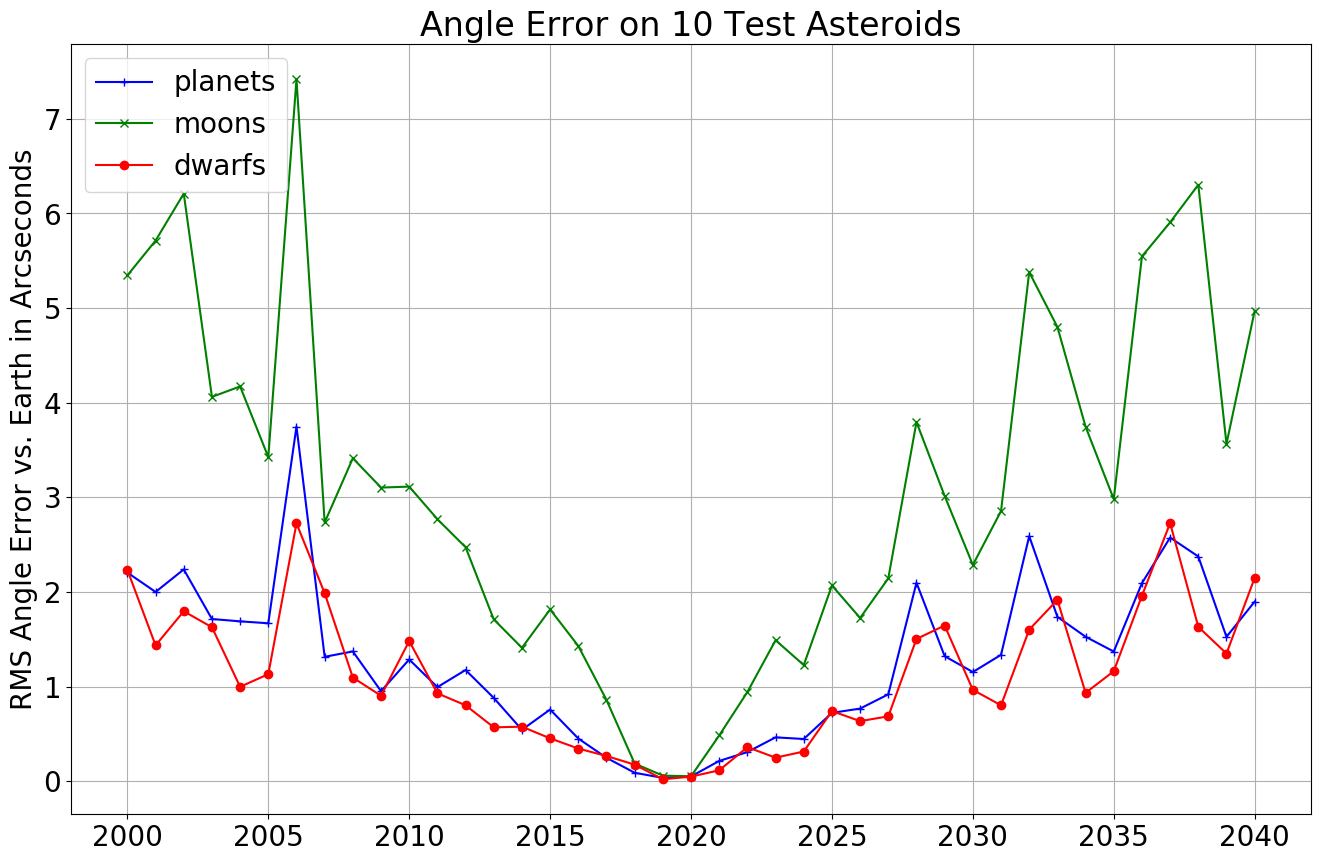
\includegraphics[width=1.0\textwidth]{sim_pos_error_comp.png}
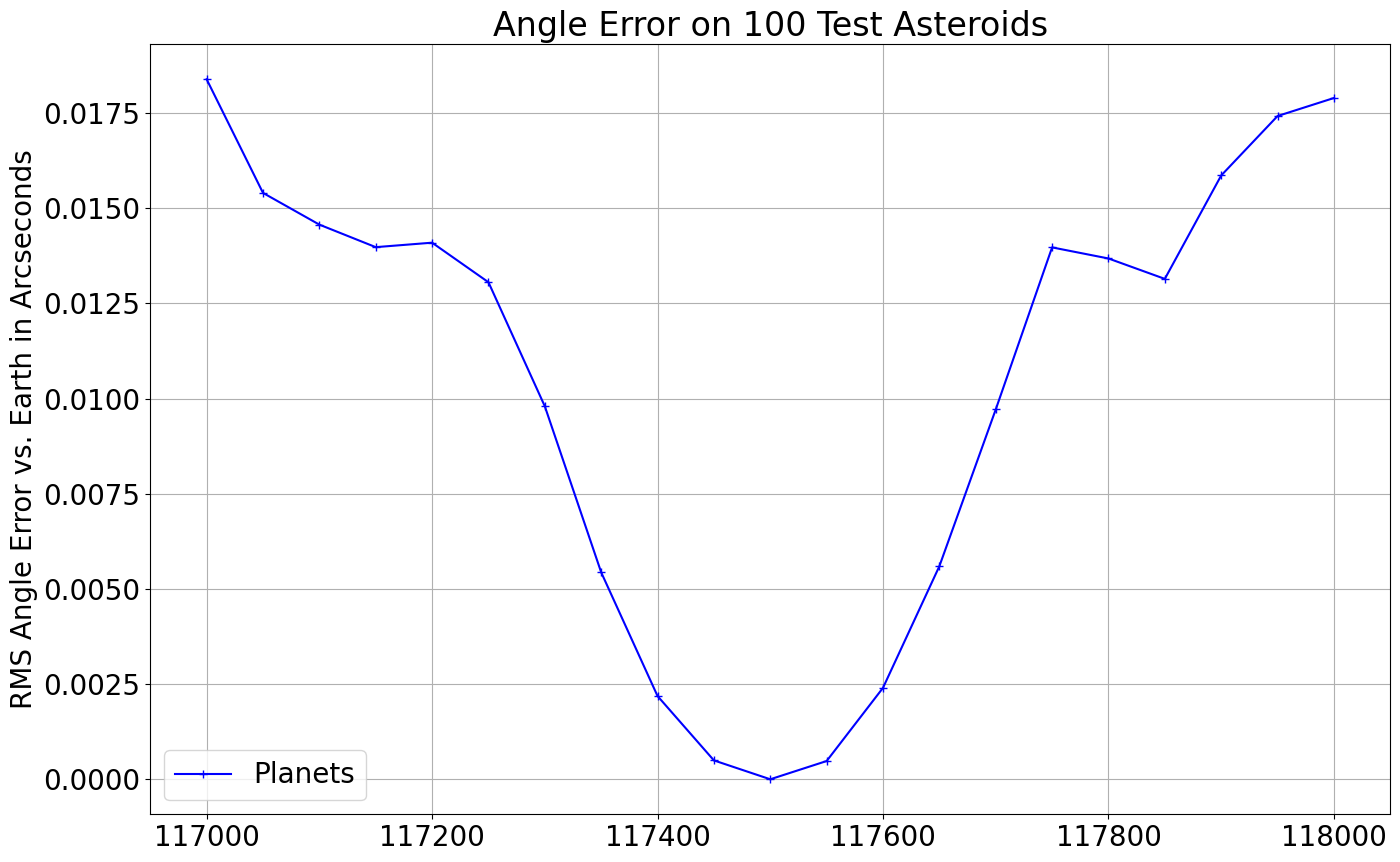
\includegraphics[width=1.0\textwidth]{sim_ang_error_comp.png}
\caption{Position and Angle Error of 10 Test Asteroids. \\
My integration is compared to positions extracted from Horizons at 40 dates from from 2000 to 2040.}
\end{center}
\end{figure}
If we focus on a plausible window of $\pm 5$ years around 2020, we can see that the selected planets integration is extremely accurate.
Angular errors 5 years out are on the order of $0.5$ arc seconds.

\section{Efficient Integration of All Known Asteroids}
\label{section_integrate_known_asteroids}

\section{Integration of Kepler Two Body Problem in Tensorflow}
\label{section_kepler_two_body_tensorflow}


\chapter{Predicting Directions from Positions}\label{ch:2}
\section{Introduction}
% \blindmathtrue\blindtext

\section{Potential outcomes framework}
% \label{sec:potent-outc-fram}
% \blindmathtrue\blindtext\footnote{Footnotes are single-spaced.
%   \blindtext}\footnote{Space between foonotes is doublespaced. \blindtext}

% \section{Conclusion}
% I conclude that:
% \blinditemize


% \chapter{Searching for Asteroids}\label{ch:3}
% \section{Introduction}
\label{section_ztf_intro}
Zwicky Transient Facility (\href{https://www.ztf.caltech.edu/}{ZTF}) is a time-domain survey of the northern sky
that had first light at Palomar Observatory in 2017.  It is run by CalTech.
My advisor Pavlos suggested it as a data source for this project.
The ZTF dataset has two major advantages for searching for asteroids:
\begin{itemize}
\item ZTF gives a wide and fast survey of the key, covering over 3750 square degrees an hours to a depth of 20.5 mag
\item A machine learning pipeline has been developed to classify a subset of ZTF detections that are classified as probable asteroids
\end{itemize}
The data set I analyze here consists of all ZTF detections that were classified as asteroids.
Data on each detection include:
\begin{itemize}
\item \textbf{ObjectID} an identifier of the likely ojbect associated with this detection; multiple detections often share the same ObjectID
\item \textbf{CandidateID} a unique integer identifier of each detection
\item \textbf{MJD} The time of the detection as an MJD
\item \textbf{RA} The right ascension of the detection
\item \textbf{Dec} The declination of the detection
\item \textbf{mag} The apparent magnitude of the detection
\end{itemize}
Available data also includes a number of additional fields that were not used in the analysis.

\href{https://github.com/alercebroker}{ALeRCE} (Automatic Learning for the Rapid Classification of Events) is an astronomical data broker.
ALeRCE provides a convenient API to access the ZTF asteroid data, which can be installed with \tty{pip}.
I used ALeRCE on this project to download the ZTF asteroid data set.

\section{Exploratory Data Analysis of ZTF Asteroid Data}
\label{section_ztf_eda}
Before plowing into the search for new asteroids, I conducted an exploratory data analysis (EDA) of the ZTF asteroid dataset.
This can be followed interactively in the Jupyter notebook \tty{05\_ztf\_data.ipynb}.
I took a download of the data running through 26-Feb-2020.
The first detection is on 01-Jun2018.
The dataset contains 5.69 total detections.  
The volume of detections increases very significantly beginning in July 2019; 
for practical purposes the dataset consists of 8 months of detections spanning July 2019 through February 2020.

\begin{figure}[hbt!]
\begin{center}
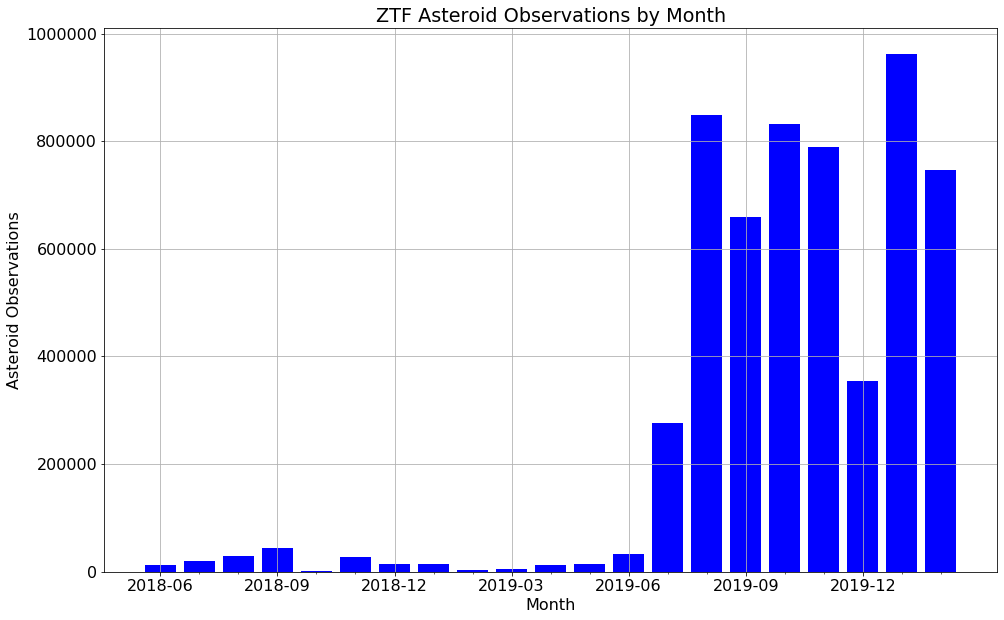
\includegraphics[width=0.85\textwidth]{../figs/ztf/ztf_ast_per_month.png}
\caption{ZTF Asteroid Detections per month}
\end{center}
\end{figure}

\begin{figure}[hbt!]
\begin{center}
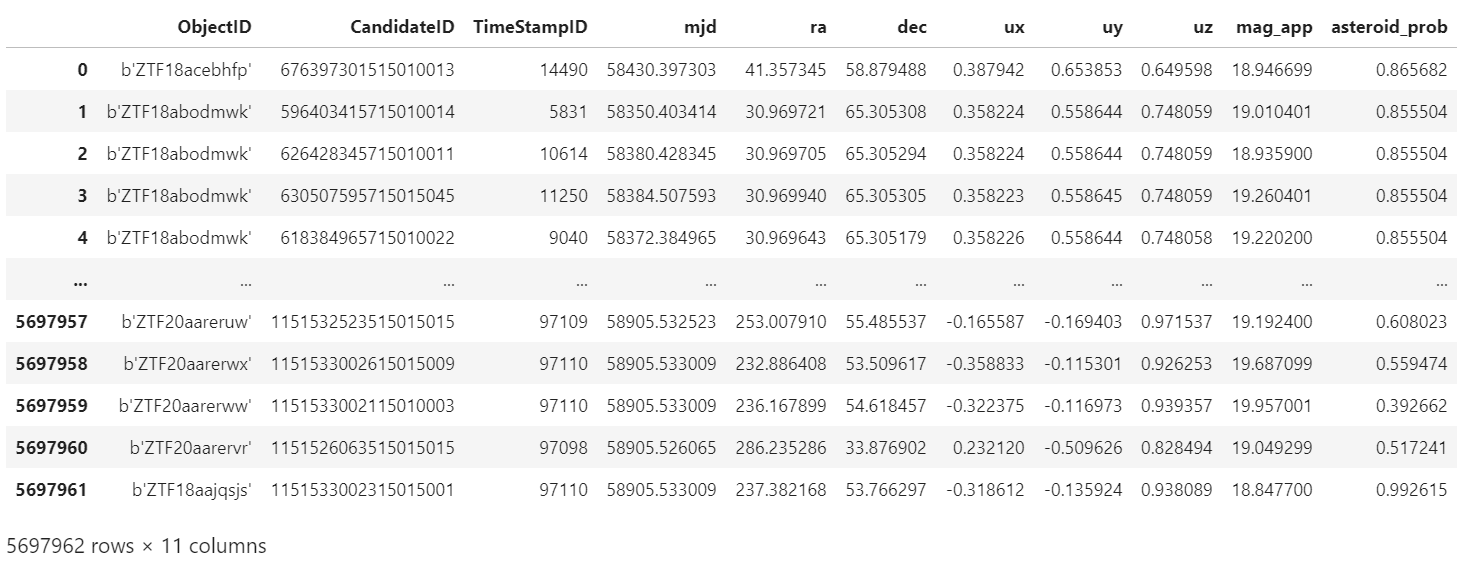
\includegraphics[width=1.0\textwidth]{../figs/ztf/ztf_dataframe.png}
\caption{Preview of Pandas DataFrame of ZTF Detections}
\end{center}
\end{figure}

The fields \tty{mjd}, \tty{ra}, \tty{dec}, and \tty{mag\_app} are part of the original dataset.
I have populated the columns \tty{ux}, \tty{uy} and \tty{uz} by running \tty{radec2dir} on the quoted RA/Dec from ZTF.

Here is a chart showing the distribution of apparent magnitudes in the ZTF detections.
It's shown on a log scale because there are so many more detections around the peak 19.5
than at the brightest (10) and and dimmest (22) magnitudes. 
\begin{figure}[hbt!]
\begin{center}
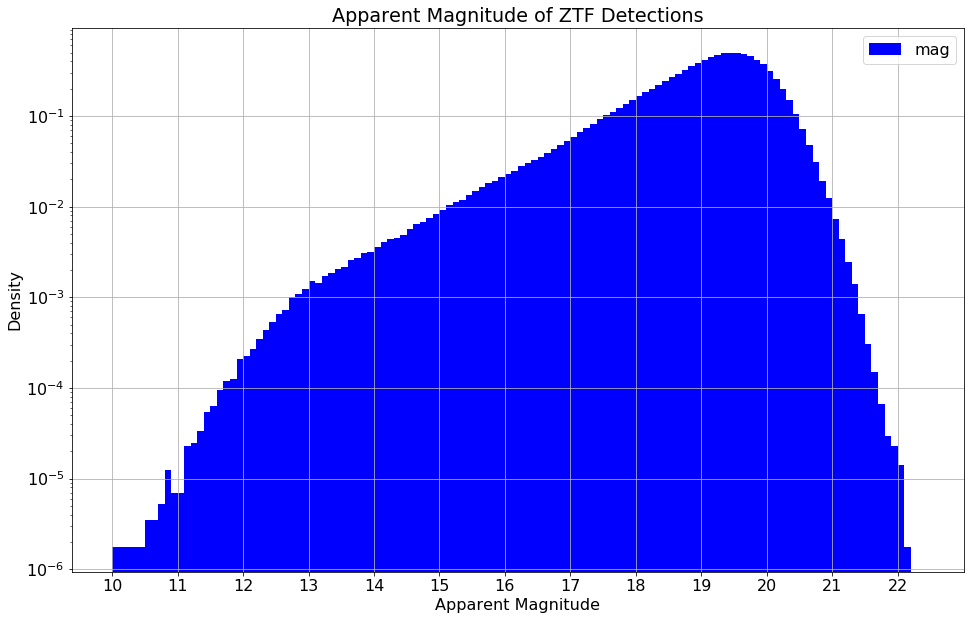
\includegraphics[width=0.85\textwidth]{../figs/ztf/apparent_mag.png}
\caption{Apparent Magnitude of ZTF asteroid detections.}
\end{center}
\end{figure}
\clearpage

\section{The Angular Distance Bewteen two Directions $\vec{u}_1$ and $\vec{u}_2$}
\label{section_ztf_angle_diff}
A recurring task in this thesis to compute the angular distance bewteen two directions on the unit sphere.
If $\uvec_1$ and $\uvec_2$ are on the unit sphere, we can compute their Cartesian distance $s$ in the usual way,
$$ s = \norm{\uvec_2 - \uvec_1}$$
$s$ will be in the interval $[0, 2]$.
We would also like to know the angular distance $\theta$ of the shortest path 
on the surface of the sphere (geodesic) connecting these two points.
On Earth, this would be analogous to the length of the great circle route by airplane between two cities.
Here is a simple picture demonstrating the derivation of the formula relating $s$ and $\theta$.
\begin{figure}[hbt!]
\begin{center}
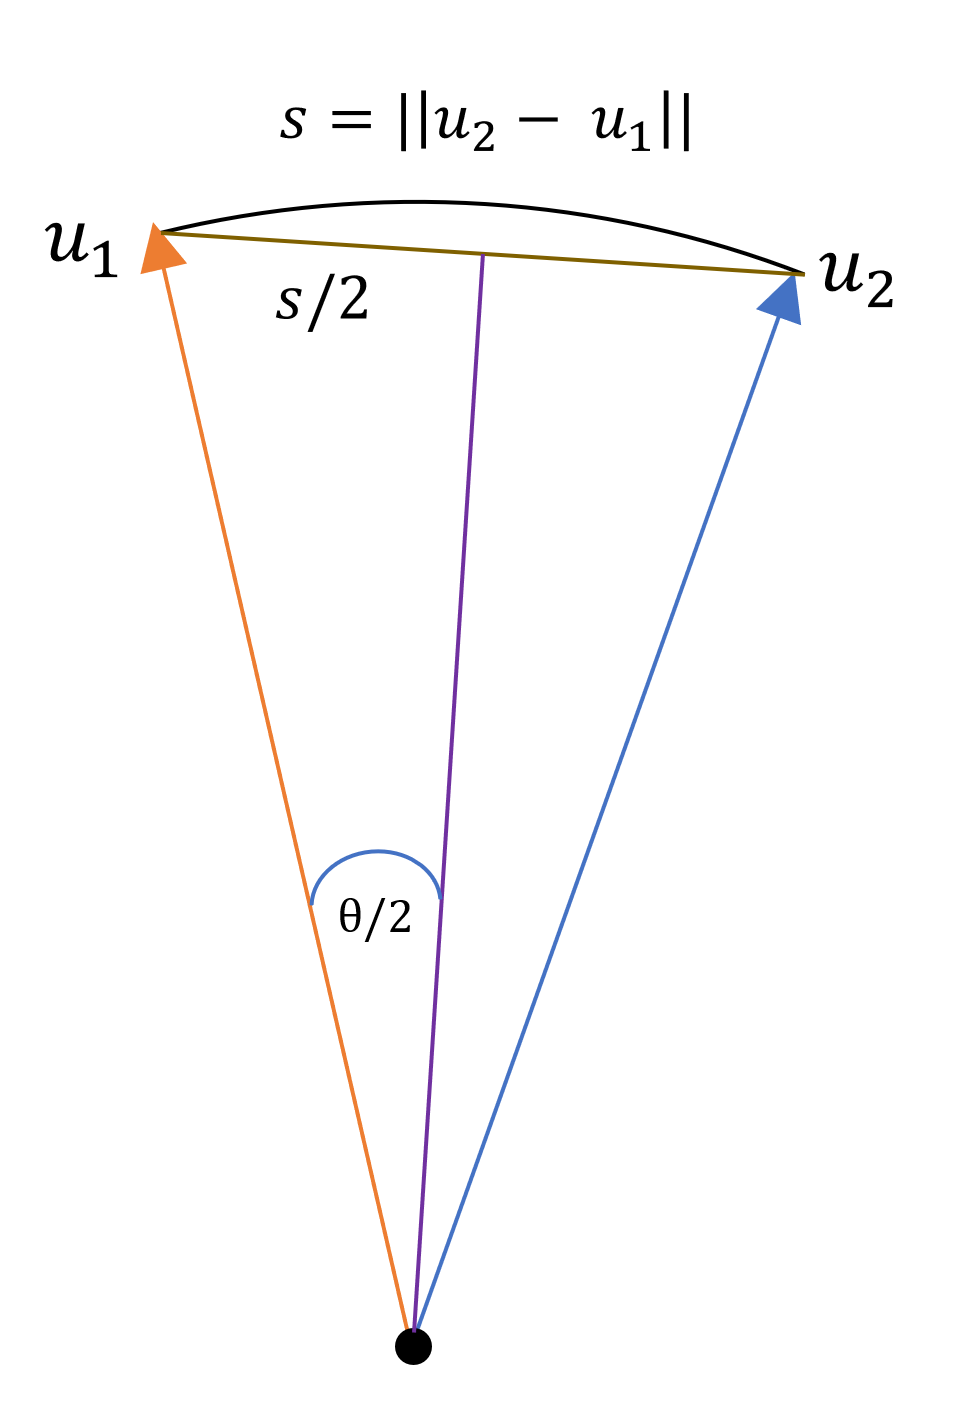
\includegraphics[width=0.3\textwidth]{../figs/misc/angular_distance.png}
\caption{The angular distance between two directions on the unit sphere.}
\end{center}
\end{figure}
The two directions are shown as arrows pointing up.
The distance between them $s$ is bisected by a line segment from the center of the sphere.
This forms a right triangle with hypotenuse $1$ and side length $s/2$ opposite angle $\theta/2$.
We thus obtain the formulas
\begin{align*}
\sin (\theta / 2) &= s / 2 \\ 
\theta &= 2 \arcsin (s / 2) \\
s &= 2 \sin \theta (\theta / 2)
\end{align*}
This function is implemented in \tty{astro\_utils} as \tty{deg2dist} and \tty{dist2deg} to convert between degrees and Cartesian distance in either direction.

\section{Finding the Nearest Asteroid to Each ZTF Detection}
\label{section_ztf_nearest_ast}
We now have in principle all the tools required to find which asteroid was closest in angular distance to each ZTF observation.
To recap the key steps, each ZTF observation is converted from a RA/Dec to a direction in the BME.
The position of Earth and each of the 733,489 catalogued asteroids are integrated as of the objervation time, and the direction bewteen them is calculated.
There are a few problems with the brute force approach implicitly suggested above.
We have 5.7E6 detections and 7.3E5 catalogued asteroids for a total of 4.16E12 (4.16 billion) interactions.
Even if we work in single precision with 4 bytes per float, we need 12 bytes for a 3D direction difference translating to about 50 GB to load the matrix in memory.
The bigger problem is that a brute force integration of all the asteroids at the MJDs of the all 5.7 million observations would be brutally slow.

Fortunately there are a few simple tricks we can use that together make this problem tractable.
The ZTF detections come from a series of images taken through the same telescope, so they come in blocks made at the same time.
The 5.7 million rows share ``only'' 97,111 distinct MJDs.
We also don't need to re-integrate the asteroid orbits.
We've already done a high precision numerical integration at a 1 day frequency and saved the results into \tty{numpy} arrays in blocks of 1,000 asteroids at a time.
Our entire data span only 635 days.  
Loading one block of 1,000 asteroids therefore has only 3.81 million numbers (635 days x 1,000 asteroids x 6 numbers per integration point).

The code to load the basic ZTF data from ALeRCE is included in the module \tty{ztf\_data.py}.
The main function used by consumers is \tty{load\_ztf\_det\_all}, which loads a cached copy of all the available detections from the local disk.
The module \tty{ztf\_nearest\_ast.py} contains a Python program that peforms the calculation described above.
The block size is a parameter that can be controlled from the commandline; I ended up leaving it at 1,000.
Checking back from my handwritten notes when I ran the job, it took approximately 25 hours to complete on a powerful server with 40 Intel CPU cores.
The job ended up being memory bound, maxxing out all 256 GB of available RAM on the server.
The initial job described above writes only computes the nearest asteroid in a block of 1,000 asteroids.
A second reduction operation is then carried out to find the nearest asteroid overall.
To limit memory usage, this was done in two steps.
First, I took 16 chunks of 1,000 at a time to find the nearest asteroid in a block of 16,000 to each detection.
Then I combined all the blocks of 16,000 (about 46) to generate one file with the nearest asteroid.

The work of splining the asteroid directions is done in the module \tty{asteroid\_dataframe.py}.
It includes functions to load the asteroid data from disk; spline the positions and velocities to the requested dates;
and compute the astrometric directions to these splined positions and velocities.
The module \tty{ztf\_ast} does the work of comparing a block of ZTF observations to a block of splined asteroid directions and finding the nearest one.
Once these calculations have been done once, you don't need to worry about them unless you are adding a new block of ZTF data.
Consumers can load the assembled DataFrame including the nearest asteroid number and distance with 
a single call to \tty{load\_ztf\_nearest\_ast} which is defined in \tty{asteroid\_dataframe}.
For the motivated reader who would like a detailed an interactive review of all these calculations, please see the Jupyter notebook \tty{04\_asteroid\_dataframe.ipynb}.
It includes tests comparing my splined outputs of daily data to Horizons data downloaded at a 3 hour interval.

\begin{figure}[hbt!]
\begin{center}
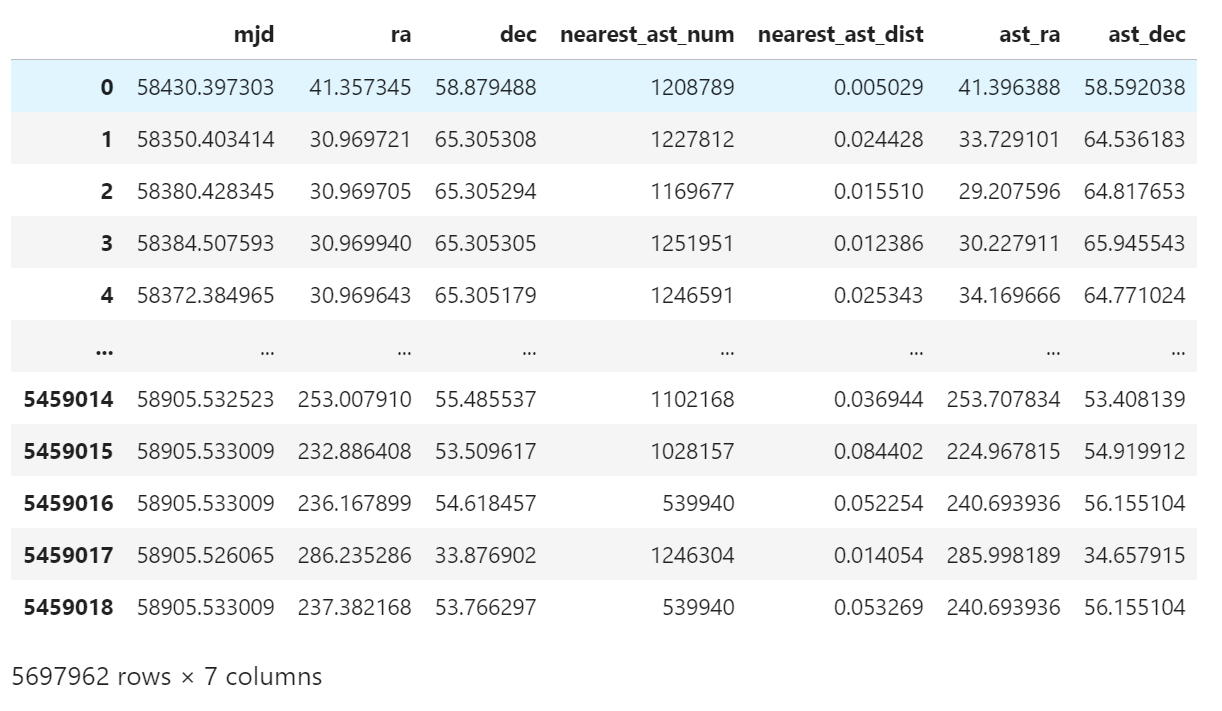
\includegraphics[width=0.9\textwidth]{../figs/ztf/ztf_nearest_ast_dataframe.png}
\caption{Preview of Pandas DataFrame of ZTF Detections Including Nearest Asteroid}
\end{center}
\end{figure}
% \clearpage

One natural question is how the brightness of the nearest asteroid to a detection varies between hits and misses.
The chart below plots two histograms of the absolute magnitude parameter H for the nearest asteroid to each ZTF detection.
Hits are shown in blue, misses in reds.
The distribution of both charts is similar, but there is a noticeable tilt 
in favor brighter asteroids being hits and dimmer asteroids being misses.
This is exactly what we would expect; 
the nearest asteroids when the distance is over the hit threshold are close to a random sample of the asteroids.
The blue series though is not a random sample, it's a sample conditional on the detection matching a real asteroid.
The brightest asteroids are more likely to be successfully detected.

\begin{figure}[hbt!]
\begin{center}
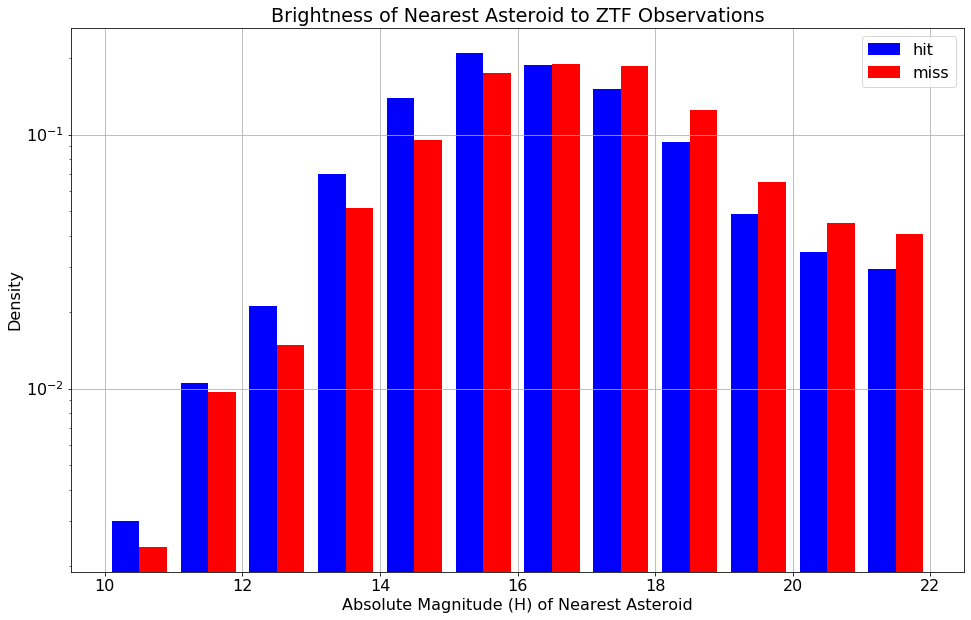
\includegraphics[width=1.0\textwidth]{../figs/ztf/nearest_ast_brightness.png}
\caption{Magnitude H of Nearest Asteroid to Each Detection\\
Hits are shown in blue, misses in red; a hit is a detection within 2.0 arc seconds of its expected direction.\\
The hits are slightly but noticeably tilted in favor of brighter asteroids.}
\end{center}
\end{figure}

I would like to take a step back and review what has been presented thus far.
Over 4 billion interactions between a ZTF asteroid detection and the predicted position of a known asteroid in the sky have been generated.
These have been filtered to associate each ZTF detection with the known asteroid it is nearest to.
This is a powerful enrichment of the original ZTF dataset, and might open the door to some additional work in the future.
For example, it could be used to create a bulk data set linking the original image files to the asteroids they belong to.
This could in turn be used to refine the machine learning pipeline used to classify detections and guess when they belong to the same object.

\section{Analyzing the Distribution of the Distance to the Nearest Asteroid}
\label{section_nearest_ast_distribution}
In this section I explore the statistical distribution of the Cartesian distance between observations and the nearest asteroid.
I compare the observed distribution of this distance to the theoretical distribution we would obtain 
if either our observed or predicted directions were distributed uniformly at random on the sphere.

\begin{figure}[hbt!]
\begin{center}
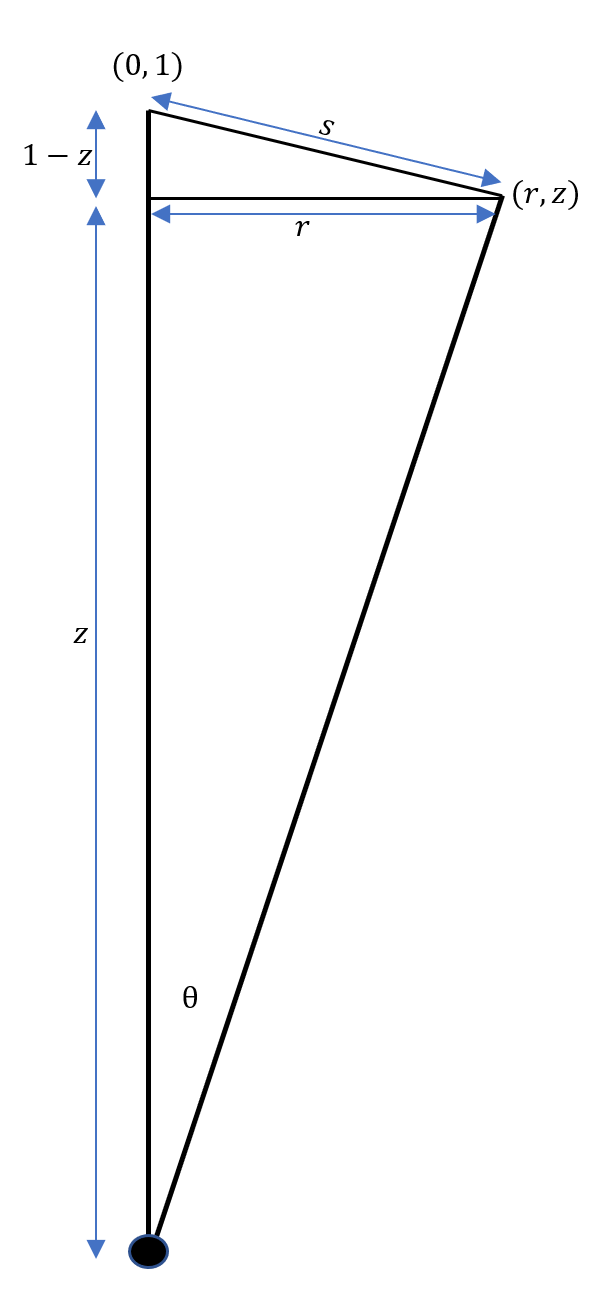
\includegraphics[width=0.36\textwidth]{../figs/misc/orange_slice.png}
\caption{Distance between an observation at the north pole and an arbitrary point.\\
The observed direction $\uobs$ is assumed w.l.o.g. to be at the north pole $(0, 0, 1)$.\\
The predicted direction $(x,y,z)$ is rotated in the $xy$ plane to to $(r, 0, z)$ \\
The Cartesian distance to from the observation to $(r,z)$ is $s$, the hypotenuse of a right triangle with sides $1-z$ and $r$.}
\end{center}
\end{figure}
Suppose without loss of generality that the observed direction is at the north pole, i.e. $\uobs = (0, 0, 1)$.
Suppose that the direction we predict is $(x, y, z)$.
Observe that the problem is symmetric about the $z$ axis, so we can rotate the problem into 
the plane containing the center, the north pole, and our guess.
Let $r^2 = x^2 + y^2$ be the squared distance from the $z$ axis to our guess.
This configuration is shown in the diagram above.
We can can relate the Cartesian distance $s$ to the height $z$ of our guess with the following simple observations.\\
$(x, y, z)$ lies on the surface of a sphere, so $x^2 + y^2 + z^2 = 1$.\\
$r^2 = x^2 + y^2$ by definition, so $r^2 = 1 - z^2$.\\
In our diagram, we can see that $s$ is the hypotenuse of a right triangle whose other two side have length $r$ and $1-z$.
Applying the Pythagorean Theorem, we find $s^2 = (1-z)^2 + r^s$. \\
This simplifies to
\begin{align*}
s^2 &= 2(1-z) \\
z &= 1 - \frac{s^2}{2}
\end{align*}
It turns out that this is a very useful parameterization because there is an elegant parameterization 
of the differential solid angle $d\Omega$ in terms of $dz$.
When surface integrals of a sphere are taught in introductory multivariate calculus courses, 
students are most likely to be exposed only to the surface element in spherical coordinates $(r, \theta, \phi)$ which is
$d\Omega = \sin \theta d\theta d\phi$.
See, e.g. \href{https://en.wikipedia.org/wiki/Spherical_coordinate_system}{Wikipedia - integration in spherical coordinates}.
But the parameterization in terms of the height $z$ along the $z$ axis is especially clean and convenient on this problem.\\
Observe that $z = \cos \theta$ so $dz = |- \sin \theta| d\theta = \sin \theta d\theta$.  
We take absolute values because this is an application of the change of variables formula and measures are always positive. \\
Substituting this expression for the surface element, we obtain
$$ d\Omega = dz \cdot d\phi$$
I call this result the ``orange slicing theorem.''
It tells you that if you slice an orange into horizontal slices, the amount of rind on each slice will be equal to $2 \pi$ times the height of the slice.

As a quick sanity check of this result, let's see if we can recover that the surface area of  the unit sphere is $4 \pi$:
$$ A = \int_{z = -1}^{1} \int_{\phi=0}^{2 \pi} d \phi dz = 2 \pi \int_{z = -1}^{1} dz = 4 \pi$$
We can now write the probability density function (PDF) for any function that can be expressed in terms of $z$.
Think of $Z$ as a random variable now.  The above result shows that when $Z$ is uniformly distributed on the unit sphere,
$$Z \sim \Unif(-1, 1)$$
Previously we showed that $z = 1 - s^2 / 2$.
This is a very useful result; it tells us that if we treat the squared distance as a random variable $S^2$, then it is uniformly distributed on $[0, 2]$.
Even more usefully, the conditional distribution of $S^2$, conditioned on $S^2 \le \tau^2$, is also uniform:
$$ S^2 | S^2 \le \tau^2 \sim \Unif(0, \tau^2)$$
If we apply a threshold distance $\tau$ and only consider predicted directions that are within Cartesian distance $\tau$ of an observation,
then the condtional distribution of the relative distance over the threshold squared is uniform on $[0, 1]$.
In mathematical notation instead of words, \\ 
Let $\upred$ be a random variable distributed uniformly on the unit sphere.\\
Let $S = \norm{\upred - \uobs}$ be the Cartesian distance between $\upred$ and $\uobs$. \\
Let $\tau$ be a threshold distance in [0, 2].\\
Let $V = S^2 / \tau^2$ be the relative squared distance of on observation vs. the threshold.\\
Then the conditional distribution of $V$, conditional on $S < \tau$ (equivalently $V < 1$) is
% $$V \sim \Unif(0, 1)$$

This describes the conditional distribution of distances we would see if we guessed one random direction in the sky.
But in this experiment, we are picking $733,489$ directions in the sky, one for each of the catalogued asteroids.
Then we are taking the minimum of these distances.
Can we still write down the conditional distribution of our nearest guess 
if they were indepedently and identically distributed (i.i.d.) at random as above?

Yes - Statistics 110 to the rescue!
Theorem 8.6.4: PDF of Order Statistics \cite{BH} states that if $X_1, \ldots X_n$ are i.i.d. continuous random variables
with PDF $f$ and CDF $F$, then the PDF of the $j$th order statistic (the $j$th smallest item $X_{(j)}$) is
$$f_{X_{j}})(x) = n \cdot {{n-1}\choose{j-1}} f(x) \cdot F(x)^{j-1} \cdot (1 - F(x))^{n-j}$$
In the special case that the $X_j$ are uniforms, this simplifies further (Example 8.6.5: Order statistics of Uniforms) \cite{BH}:\\
Let $U_1, \ldots U_n$ be i.i.d. $\Unif(0,1)$.
Then the distribution of $U_{j}$ is the Beta distribution,
$$U_{(j)} \sim \Beta(j, n-j+1)$$
The minimum is the order statistic of $j=1$, so
$$U_{(1)} \sim \Beta(1, n)$$ 

Let us now apply this theoretical result to compare our distribution of distances to what we would have obtained if 
we were randomly throwing darts into the sky so to speak.
The module \tty{ztf\_data\_viz} includes these calculations as well as the generation of charts.
\tty{cdf\_nearest\_dist} computes the theoretical CDF using the approach described above.
In the charts below, I will demonstrate that 2.0 arc seconds is a good threshold for classifying detections as ``hits'' against known asteroids.
For now, please treat it as a parameter I have chosen to demonstrate that these calculations work and are getting
astronomically more hits (no pun intended) than would arise from random chance.

Out of 5.69 million detections, 3.75 million (65.71\%) are within 2.0 arc seconds of the nearest catalogued asteroid.
The theoretical beta distribution says that if the predicted directions were distributed uniformly at random,
we would expect only 98 hits or 0.0017\% of the total be this close.
The immediate conclusion is that this whole set of calculations is working with a tolerance no worse than 2.0 arc seconds.

We can get a better intuition for what's happening by visualizing the histogram of distance to the nearest asteroid.
I initially plotted these against the percentile of the theoretical distribution; 
these plots would be a flat line with density 1 if the predicted directions were uniformly at random.
I found however that a simple plot of frequency vs. distance in arc seconds is easier to interpret 
once you've done the statistical analysis that the results are not due to chance.
Here is a plot showing hits inside a threshold of 2.0 arc seconds:
\begin{figure}[hbt!]
\begin{center}
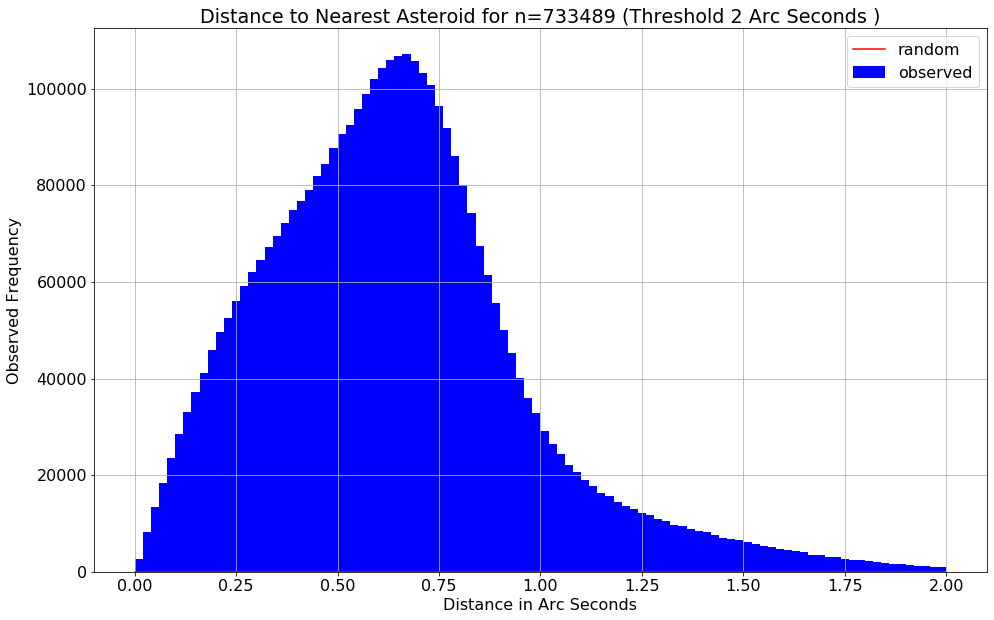
\includegraphics[width=1.0\textwidth]{../figs/ztf/nearest_ast_hist_dist.png}
\caption{Histogram of angular distance from each ZTF detection to the nearest asteroid in arc seconds.\\
These account for 65.57\% of the total data set.\\
The number of expected detections due to random chance is shown in red; it is visually indistinguishable from zero on the chart.}
\end{center}
\end{figure}

Here are two additional plot to visualize the distribution of distances between ZTF detections and the nearest known asteroid.
The first shows the absolute density in hits per square degree.
The second show the relative density of hits per square degree over what would have been expected
from the minimum of 733,489 guesses distributed uniformly at random on the sphere. \\
These charts seemed to have a shape that could be roughly approximated in a one parameter distribution as exponential.
They led me to propose a mixture model and log likelihood optimization objective function that I will describe in the next section
\begin{figure}[hbt!]
\begin{center}
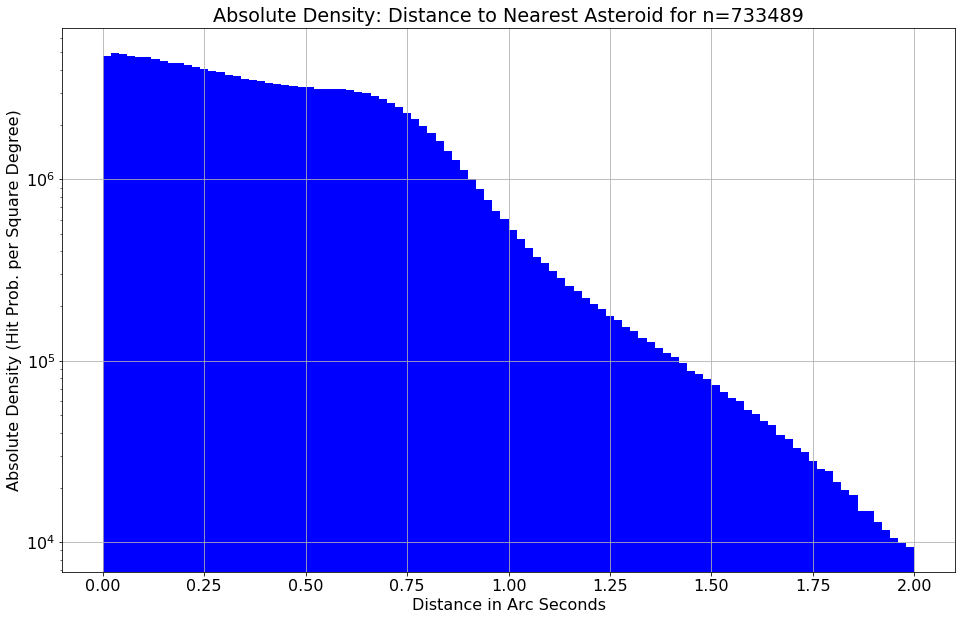
\includegraphics[width=1.0\textwidth]{../figs/ztf/nearest_ast_hist_dens_abs.png}
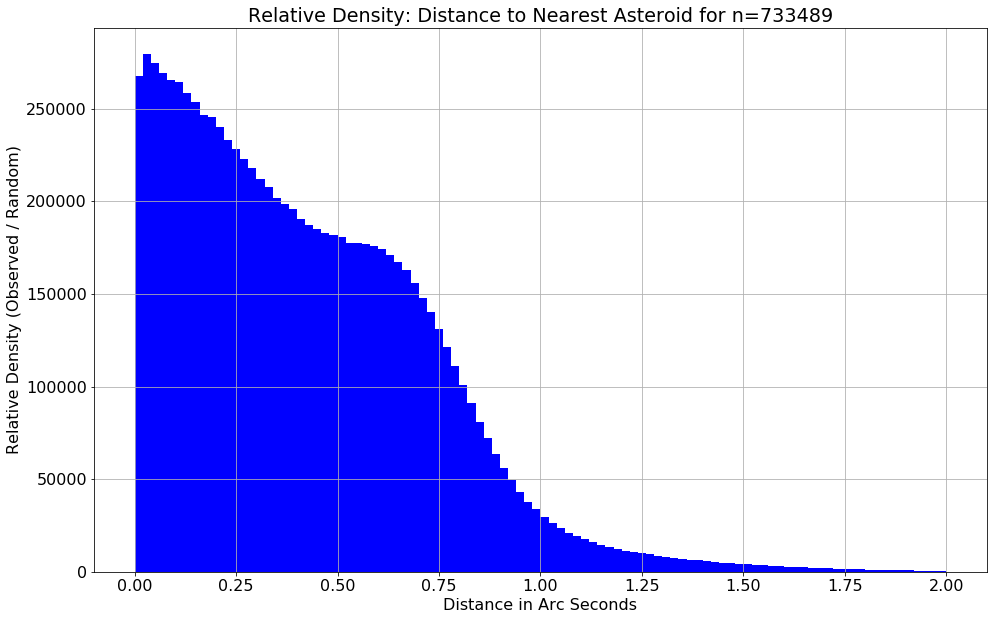
\includegraphics[width=1.0\textwidth]{../figs/ztf/nearest_ast_hist_dens_rel.png}
\caption{Density of hits for distance between ZTF detections and the nearest known asteroid. \\
The first chart shows the absolute density in hits per square degree.\\
The second chart shows the relative density of this over the baseline if the guesses were distributed randomly.}
\end{center}
\end{figure}
\clearpage

How many asteroids in the catalogue have enough detections in the ZTF dataset that we would have 
a sporting chance to recover their orbital elements from these observations alone?
Suppose for the sake of discussion that the number is $n=20$.
There are 63,746 asteroids with 20 or more hits at 2.0 arc seconds.
If we required only $n=10$ hits to recover the orbital elements, we could do it for 100,508 asteroids.\\
We can visualize this by plotting the cumulative frequency of close observations on the $y$ axis vs. hit count on the $x$ axis:
\begin{figure}[hbt!]
\begin{center}
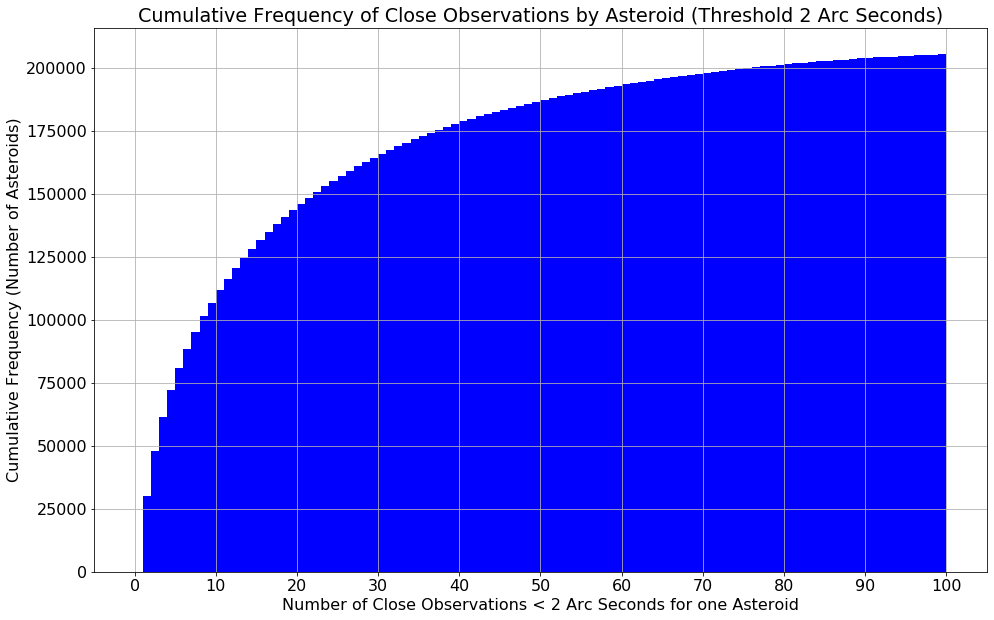
\includegraphics[width=1.0\textwidth]{../figs/ztf/nearest_ast_cum.png}
\caption{Cumulative frequency of asteroids by number of close observations < 2.0 arc seconds. \\
There are 63,746 asteroids with 20 or more close matches and 100,508 asteroids with 10 or more close matches. }
\end{center}
\end{figure}
\clearpage

\section{Conclusion}
\label{section_ztf_conclusion}
I have presented in this chapter an analysis of the asteroid detections in the ZTF astronomical data set.
I have demonstrated a calculation of the nearest known asteroid to each ZTF detection 
and the angular distance from that asteroid to the detection.
I have also developed the statistical distribution of distances that would be observed 
if the predicted directions were distributed uniformly at random on the sphere.
I have shown that of 5.7 million total ZTF detections, 65.7\% of them (almost two thirds)
are within 2.0 arc seconds of the predicted direction of the nearest known asteroid.
By comparing this number of hits to the number we would expect with a random baseline,
I have provided overwheliming evidence that this entire apparatus of data and calculations is accurate 
to a tolerance on the order of 2.0 arc seconds or better.
I have provided motivation that the approximate shape of the distribution of distances decays with an exponential tail.
Finally, I have shown the fraction of the asteroid catalogue we might be able to recover as a function of the number of observations required to fit it.  
If we require $n=10$ detections to verify or update the orbital elements of a known asteroid,
then we can apply this procedure on 100,508 asteroids representing 13.70\% of the known asteroid catalogue.

%%%%%%%%%%%%%%%% BACK MATTER %%%%%%%%%%%%%%%%

% Put appendices, bibliography, and supplemental materials here

% The bibliography may be single spaced within each entry, but must be double-spaced between each entry. 
% Most bibliography styles leave space between entries, so that shouldn't be a problem.
\begin{singlespacing}
\renewcommand{\bibname}{References}

% Any bibliohgraphy style that leaves space between entries is fine
% \bibliographystyle{acm}
% \bibliography{references}
\newpage
\begin{thebibliography}{9}

\bibitem{RL-Rebound} 
Hanno Rein, Shang-Fei Liu\\
\textit{REBOUND: An open-source multi-purpose N-body code for collisional dynamics}.\\
Astronomy \& Astrophysics.  November 11, 2011.\\
arXiv: 1110.4876v2

\bibitem{RL-IAS15} 
Hanno Rein, David S. Spiegel\\
\textit{IAS15: A fast, adaptive high-order integrator for gravitational dynamics, accurate to machine precision over a billion orbits}.\\
Monthly Notices of the Royal Astronomical Society.  Printed 16 October 2014.\\
arXiv: 1405.4779.v2

\bibitem{SSD}
Murray, C. D.; Dermott, S.F. \\
\textit{Solar System Dynamics}\\
Cambridge University Press. 1999

\bibitem{BH}
Joseph Blitzstein, Jessica Hwang\\
\textit{Introduction to Probability}\\
CRC Press.  2019 (Second Edition)

\end{thebibliography}
\end{singlespacing}

% Appendices from all chapters should go at the end
% \begin{appendices}

\chapter{Appendix to Chapter \ref{ch:1}}\label{cha:append-chapt-refch:1}

\section{Auxiliary Lemmata}
Fundamental identity
\begin{equation}
  \label{eq:A}
  e^{i\pi}=-1.
\end{equation}
Equivalence relation
\begin{equation}
  \label{eq:B}
  A=B.
\end{equation}

\section{Proofs}

\chapter{Appendix to Chapter \ref{ch:3}}

\section{Proofs}

\section{Supplementary Tables and Figures}
\begin{longtable}{cc}
% Caption to appear on the first page and in the list of tables
\caption[Optional Short caption (used in list of tables)]{A long table} \label{grid_mlmmh} \\

Heading that appears & on first page only\\
\hline
\endfirsthead
\caption[]{(continued)}\\ % Caption to appear on subsequent pages. GSAS requires
                          % that if a table spills over multiple pages, it
                          % contains the (continued) label

Heading that appears & on all pages\\
\hline
\endhead
% optional footer
\hline \multicolumn{2}{r}{{Continued on next page}} \\
\endfoot
% footer to appear on tha last page (empty)
\endlastfoot

Contrary to popular & belief, Lorem Ipsum \\ is & not \\ simply &
random \\ text &. It \\ has & roots \\ in & a \\ piece & of \\ classical & Latin
\\ literature & from \\ 45 & BC \\, making & it \\ over & 2000 \\ years old. Richard & Mc \\Clintock &, a \\ Latin & professor \\ at & Hampden \\-Sydney
& College \\ in & Virginia \\, looked & up \\ one & of \\ the & more
\\obscure & Latin \\ words &, consectetur \\, from & a \\ Lorem & Ipsum \\
passage &, and \\ going & through \\ the & cites \\ of & the word in \\
classical & literature , discovered the \\ undoubtable & source. Lorem Ipsum
\\ comes & from \\ sections & 1 \\.10 &.32 \\ and & 1 \\.10 &.33 \\ of
&"de \\ Finibus & Bonorum \\ et & Malorum \\" (The & Extremes \\ of & Good \\
and & Evil \\) by & Cicero \\, written & in \\ 45 & BC \\. This & book \\ is & a
\\ treatise & on \\ the & theory \\ of & ethics \\, very & popular \\ during
&the \\ Renaissance &. The \\ first & line \\ of & Lorem \\ Ipsum, "Lorem ipsum
& dolor \\ sit & amet \\..", comes from a & line \\ in & section
1.10.32.\\
\end{longtable}


\begin{sidewaysfigure}
  \centering Supplementary figures and tables should be placed in the appendix,
  not at the end of a chapter. To rotate big tables and figures $90^{\circ}$,
  use the rotating package and the sidewaystable and sidewaysfigure
  environments. This ensures that the figure and caption get rotated, but the
  page number stays at the bottom of the page.
  \caption{Supplementary Figure}
  \label{fig:figuresup1}
\end{sidewaysfigure}

\begin{figure}[ht]
  \centering
  This is another supplementary figure.
  \caption{Another Figure}
  \label{fig:figuresup3}
\end{figure}


\end{appendices}


\end{document}
